\documentclass[8pt,aspectratio=1610]{beamer}
\usepackage[utf8]{inputenc}
\usepackage{booktabs}
\usepackage{array}
\usepackage{graphicx}
\usepackage{xcolor}
\usepackage{tikz}
\usetikzlibrary{positioning,arrows.meta,decorations.pathreplacing,calc,shadows}
\usepackage{pgfplots}
\pgfplotsset{compat=1.18}
\usepackage{amsmath}
\usepackage{amssymb}
\usepackage{amsfonts}
\usepackage{algorithm}
\usepackage{algorithmic}

\usetheme{metropolis}
\usecolortheme{wolverine}
\metroset{progressbar=frametitle,block=fill}
\setbeamertemplate{navigation symbols}{}

% Define custom colors complementing the Wolverine theme
\definecolor{maizelight}{RGB}{255, 203, 5}      % Light maize for examples
\definecolor{maizedark}{RGB}{255, 167, 0}       % Darker maize for emphasis
\definecolor{bluelight}{RGB}{0, 39, 76}         % Deep blue for blocks
\definecolor{tealaccent}{RGB}{0, 128, 128}      % Teal for variety
\definecolor{orangeaccent}{RGB}{255, 138, 51}   % Orange complement

% EDA specific colors
\definecolor{datacolor}{RGB}{33, 150, 243}      % Blue for data points
\definecolor{trendcolor}{RGB}{255, 193, 7}      % Amber for trends
\definecolor{outliercolor}{RGB}{244, 67, 54}    % Red for outliers
\definecolor{featurecolor}{RGB}{76, 175, 80}    % Green for features

% Customize block colors
\setbeamercolor{block title}{bg=bluelight,fg=white}
\setbeamercolor{block body}{bg=bluelight!10,fg=black}

% Example blocks in complementary maize
\setbeamercolor{block title example}{bg=maizelight,fg=black}
\setbeamercolor{block body example}{bg=maizelight!15,fg=black}

% Alert blocks in orange accent
\setbeamercolor{block title alerted}{bg=orangeaccent,fg=white}
\setbeamercolor{block body alerted}{bg=orangeaccent!15,fg=black}

% Create custom colored blocks for variety
\newenvironment<>{techblock}[1]{%
  \setbeamercolor{block title}{bg=tealaccent,fg=white}%
  \setbeamercolor{block body}{bg=tealaccent!10,fg=black}%
  \begin{block}#2{#1}}{\end{block}}

\newenvironment<>{tipblock}[1]{%
  \setbeamercolor{block title}{bg=maizedark,fg=black}%
  \setbeamercolor{block body}{bg=maizedark!15,fg=black}%
  \begin{block}#2{#1}}{\end{block}}

\newenvironment<>{methodblock}[1]{%
  \setbeamercolor{block title}{bg=featurecolor,fg=white}%
  \setbeamercolor{block body}{bg=featurecolor!10,fg=black}%
  \begin{block}#2{#1}}{\end{block}}

% TikZ styles for EDA diagrams
\tikzset{
    data point/.style={circle, draw, minimum size=0.3cm, inner sep=0pt},
    normal data/.style={data point, fill=datacolor!30, draw=datacolor!70},
    outlier data/.style={data point, fill=outliercolor!30, draw=outliercolor!70},
    feature/.style={rectangle, draw, minimum width=1.5cm, minimum height=0.8cm},
    numerical/.style={feature, fill=datacolor!20, draw=datacolor!70},
    categorical/.style={feature, fill=trendcolor!20, draw=trendcolor!70},
    target/.style={feature, fill=featurecolor!20, draw=featurecolor!70},
    process arrow/.style={->, thick, blue!70},
    eda process/.style={rectangle, rounded corners, draw, fill=gray!10, minimum width=2cm, minimum height=0.6cm}
}

\title{Exploratory Data Analysis (EDA)}
\subtitle{CMSC 173 - Machine Learning}
\author{Course Lecture}
\date{}

\begin{document}

\begin{frame}
\titlepage
\end{frame}

\begin{frame}{Outline}
\tableofcontents
\end{frame}

% ========================================
% Section: Introduction
% ========================================

\section{Introduction to EDA}

\begin{frame}{What is Exploratory Data Analysis?}
\begin{columns}[t]
\begin{column}{0.48\textwidth}
\begin{block}{Definition}
\textbf{EDA} is the process of investigating datasets to summarize their main characteristics, often using statistical graphics and other data visualization methods.
\end{block}

\vspace{0.2cm}
\textbf{Primary Goals:}
\begin{itemize}
\setlength{\itemsep}{1pt}
\item \textcolor{datacolor}{\textbf{Understand}} data structure and quality
\item \textcolor{trendcolor}{\textbf{Discover}} patterns and relationships
\item \textcolor{outliercolor}{\textbf{Identify}} anomalies and outliers
\item \textcolor{featurecolor}{\textbf{Guide}} feature engineering decisions
\item \textcolor{tealaccent}{\textbf{Inform}} modeling strategy
\end{itemize}

\vspace{0.2cm}
\textbf{Key Questions EDA Answers:}
\begin{itemize}
\setlength{\itemsep}{1pt}
\item What does my data look like?
\item Is my data clean and complete?
\item What patterns exist?
\item Which features are important?
\end{itemize}
\end{column}

\begin{column}{0.48\textwidth}
\textbf{EDA Process Overview:}
\vspace{0.1cm}

\begin{tikzpicture}[node distance=0.8cm]
\node[rectangle, draw, fill=datacolor!20, text width=3cm, text centered, font=\small] (data) {Raw Data};
\node[rectangle, draw, fill=trendcolor!20, text width=3cm, text centered, font=\small, below=0.4cm of data] (explore) {Data Exploration};
\node[rectangle, draw, fill=featurecolor!20, text width=3cm, text centered, font=\small, below=0.4cm of explore] (clean) {Data Cleaning};
\node[rectangle, draw, fill=outliercolor!20, text width=3cm, text centered, font=\small, below=0.4cm of clean] (model) {Model Ready Data};

\draw[process arrow] (data) -- (explore);
\draw[process arrow] (explore) -- (clean);
\draw[process arrow] (clean) -- (model);
\draw[process arrow] (explore.east) .. controls +(right:0.8cm) and +(right:0.8cm) .. (data.east);
\end{tikzpicture}

\vspace{0.2cm}
\begin{alertblock}{Key Insight}
\textbf{EDA is iterative!} Insights from one analysis often lead to new questions and deeper investigations.
\end{alertblock}
\end{column}
\end{columns}
\end{frame}

\begin{frame}{The EDA Workflow}
\begin{center}
\begin{tikzpicture}[node distance=1.5cm, scale=0.9, transform shape]
% Main workflow nodes
\node[eda process, fill=datacolor!20] (load) {Data Loading};
\node[eda process, fill=trendcolor!20, right=of load] (inspect) {Initial Inspection};
\node[eda process, fill=featurecolor!20, right=of inspect] (clean) {Data Cleaning};
\node[eda process, fill=outliercolor!20, below=of clean] (viz) {Visualization};
\node[eda process, fill=tealaccent!20, left=of viz] (stats) {Statistical Analysis};
\node[eda process, fill=maizedark!20, left=of stats] (insights) {Insights \& Patterns};

% Arrows
\draw[process arrow] (load) -- (inspect);
\draw[process arrow] (inspect) -- (clean);
\draw[process arrow] (clean) -- (viz);
\draw[process arrow] (viz) -- (stats);
\draw[process arrow] (stats) -- (insights);

% Feedback loops
\draw[process arrow, dashed] (viz) to[bend left=20] (clean);
\draw[process arrow, dashed] (stats) to[bend left=30] (inspect);
\draw[process arrow, dashed] (insights) to[bend left=40] (load);
\end{tikzpicture}
\end{center}

\vspace{0.1cm}
\begin{columns}[t]
\begin{column}{0.32\textwidth}
\begin{techblock}{Data Loading}
\begin{itemize}
\setlength{\itemsep}{0pt}
\item Import datasets
\item Check file formats
\item Handle encoding issues
\end{itemize}
\end{techblock}
\end{column}

\begin{column}{0.32\textwidth}
\begin{methodblock}{Statistical Analysis}
\begin{itemize}
\setlength{\itemsep}{0pt}
\item Descriptive statistics
\item Correlation analysis
\item Distribution testing
\end{itemize}
\end{methodblock}
\end{column}

\begin{column}{0.32\textwidth}
\begin{tipblock}{Key Outcome}
\begin{itemize}
\setlength{\itemsep}{0pt}
\item Clean, understood data
\item Feature insights
\item Modeling strategy
\end{itemize}
\end{tipblock}
\end{column}
\end{columns}
\end{frame}

\begin{frame}{Why EDA is Critical for Machine Learning}
\begin{columns}[t]
\begin{column}{0.48\textwidth}
\begin{alertblock}{Without EDA}
\textbf{Common Pitfalls:}
\begin{itemize}
\setlength{\itemsep}{1pt}
\item \textcolor{outliercolor}{Garbage In, Garbage Out}
\item Poor model performance
\item Biased predictions
\item Overfitting to noise
\item Missing important patterns
\item Wasted computational resources
\end{itemize}
\end{alertblock}

\vspace{0.2cm}
\textbf{Statistical Foundation:}
\\
For dataset $\mathcal{D} = \{(\mathbf{x}_i, y_i)\}_{i=1}^n$:
\begin{align}
\text{Data Quality} &= f(\text{Completeness, Accuracy, Consistency}) \\
\text{Model Performance} &\propto \text{Data Quality}
\end{align}
\end{column}

\begin{column}{0.48\textwidth}
\begin{exampleblock}{With Proper EDA}
\textbf{Benefits Achieved:}
\begin{itemize}
\setlength{\itemsep}{1pt}
\item \textcolor{featurecolor}{High-quality, clean data}
\item Optimal feature selection
\item Appropriate model choice
\item Better generalization
\item Actionable insights
\item Efficient resource usage
\end{itemize}
\end{exampleblock}

\vspace{0.2cm}
\textbf{Impact Quantification:}
\\
Studies show that proper EDA can improve model performance by 15-30\% and reduce development time by 40-60\%.

\begin{center}
\begin{tikzpicture}[scale=0.7]
\draw[fill=outliercolor!20] (0,0) rectangle (2,1) node[pos=.5] {\small No EDA};
\draw[fill=featurecolor!20] (0,1.2) rectangle (3,2.2) node[pos=.5] {\small With EDA};
\node[right] at (2.1,0.5) {\small 60\% Accuracy};
\node[right] at (3.1,1.7) {\small 85\% Accuracy};
\end{tikzpicture}
\end{center}
\end{column}
\end{columns}
\end{frame}

% ========================================
% Section: Data Understanding
% ========================================

\section{Data Understanding \& Types}

\begin{frame}{Understanding Your Dataset}
\begin{center}
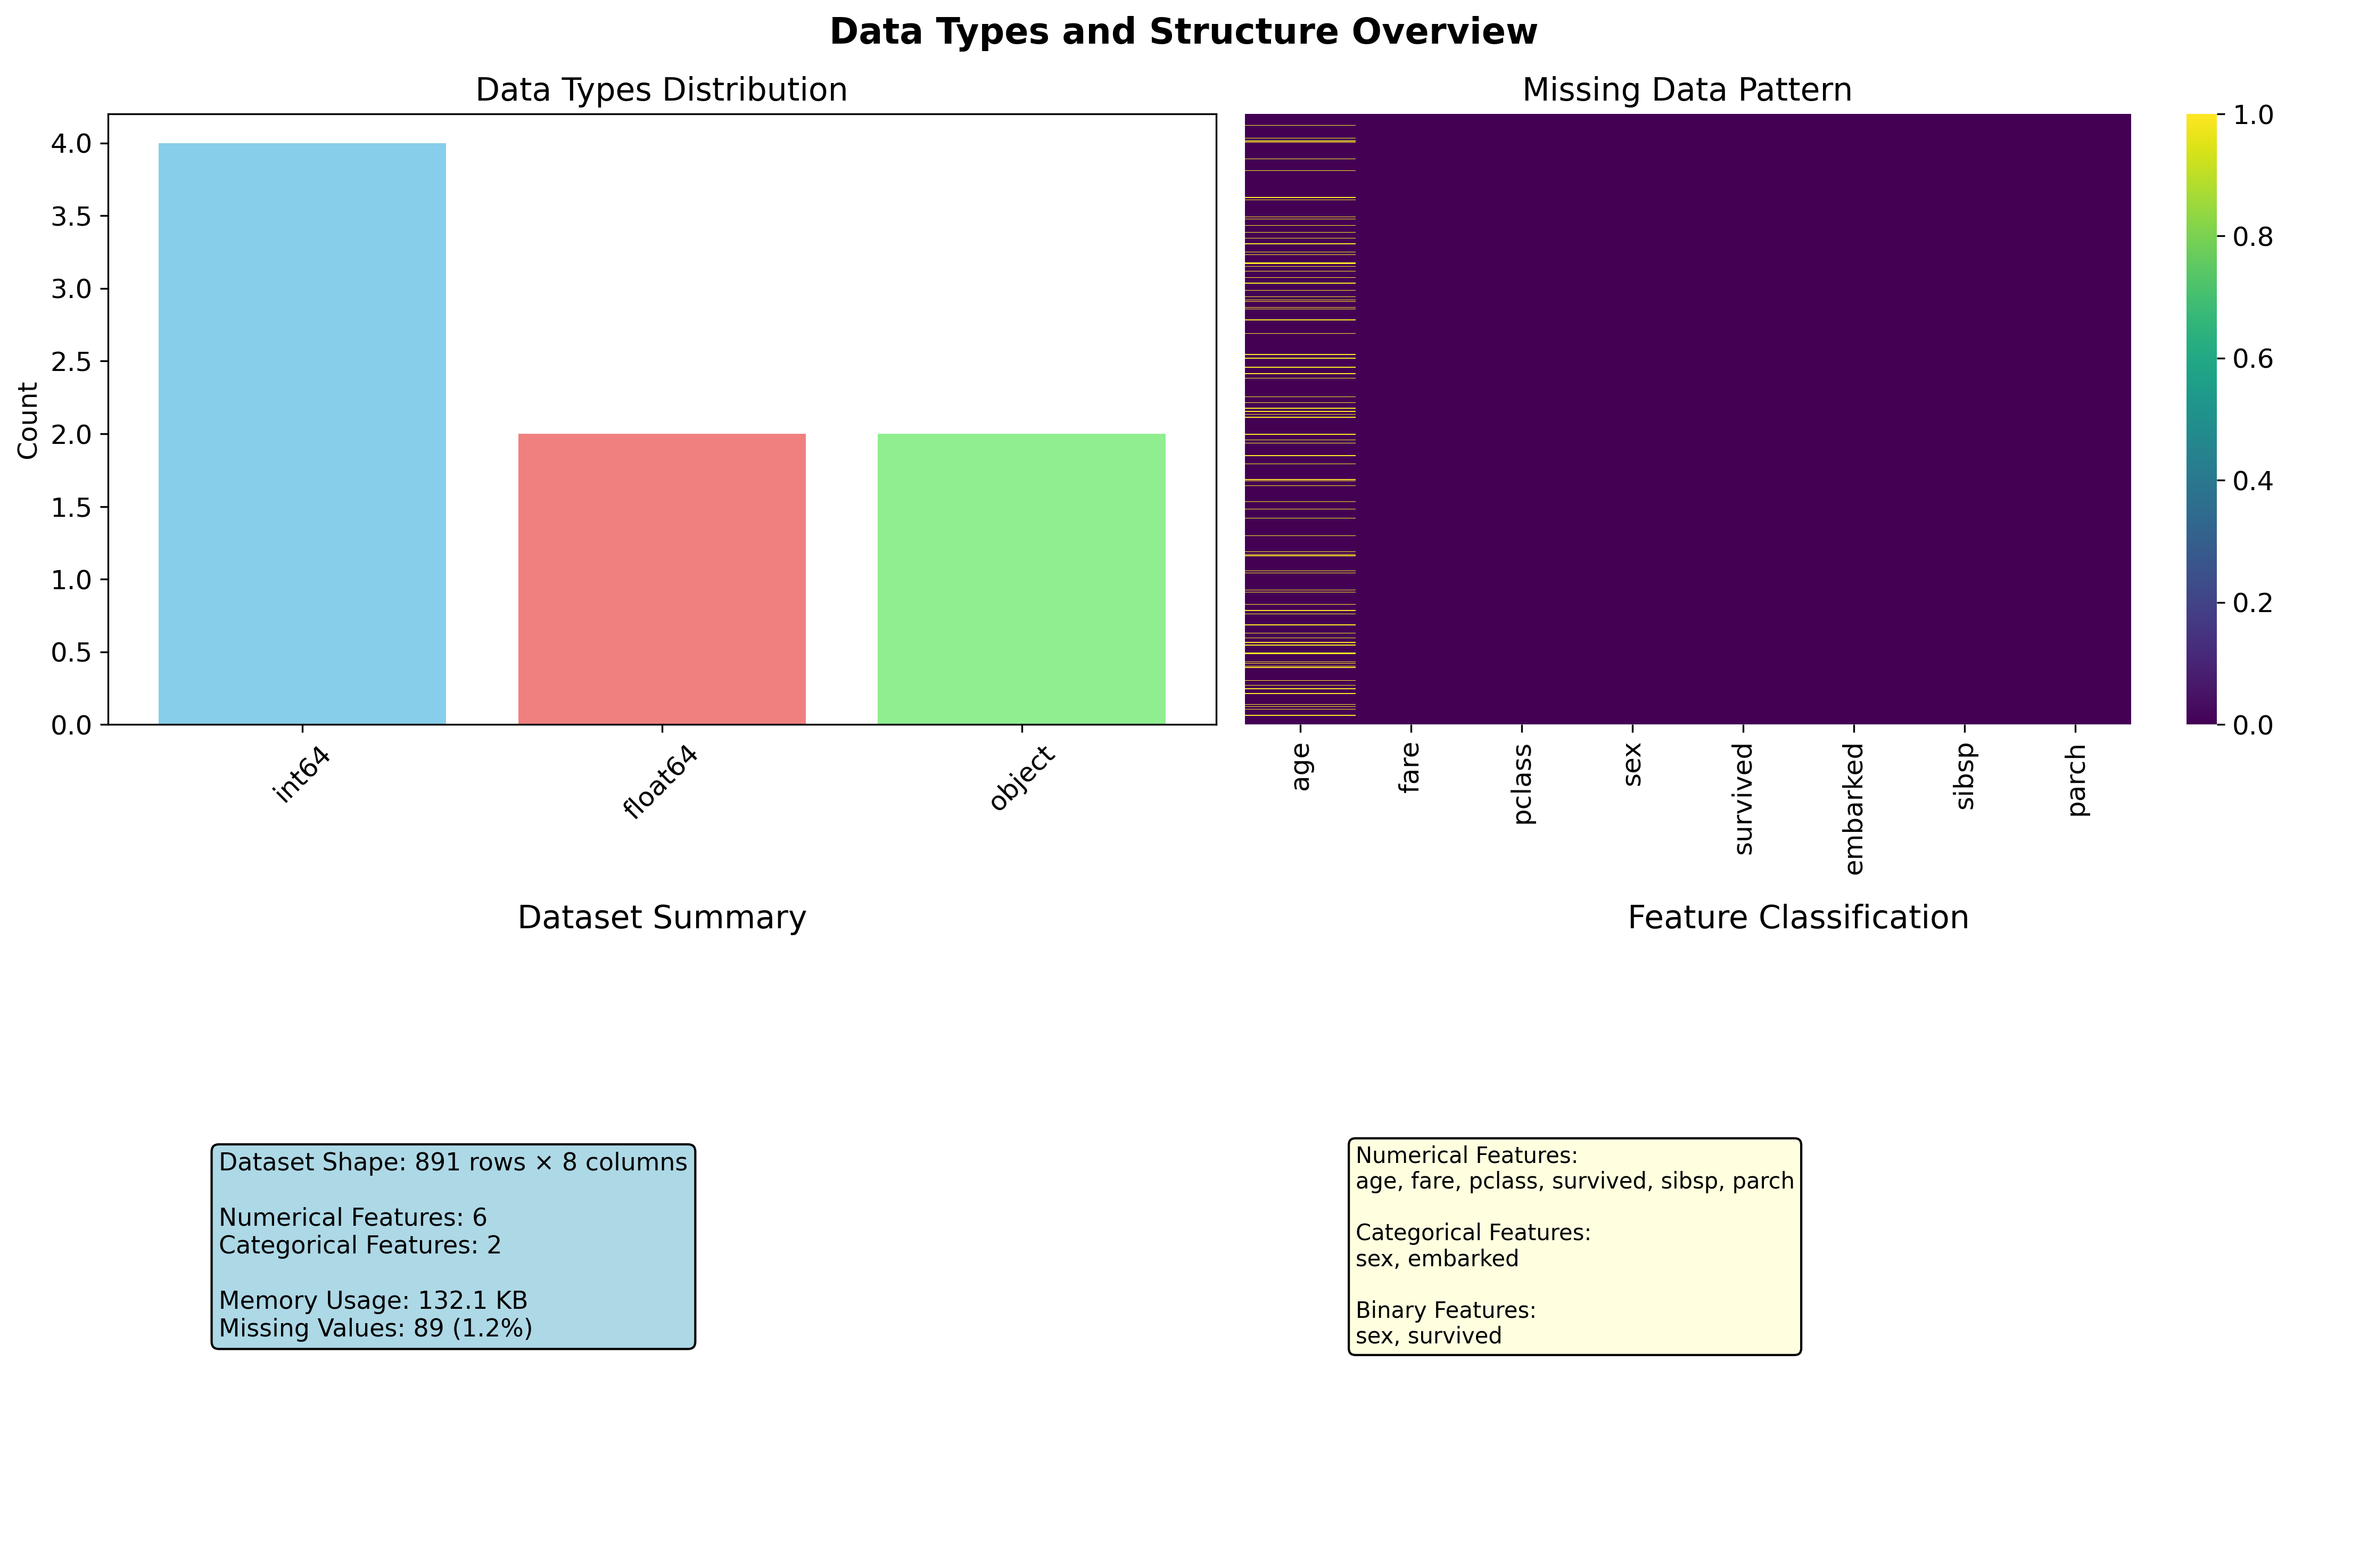
\includegraphics[width=0.9\textwidth]{../figures/01_data_types_overview.png}
\end{center}

\vspace{0.1cm}
\begin{alertblock}{First Steps}
Always start with: \texttt{df.info()}, \texttt{df.describe()}, \texttt{df.shape}, and \texttt{df.head()}
\end{alertblock}
\end{frame}

\begin{frame}{Data Types Classification}
\begin{columns}[t]
\begin{column}{0.48\textwidth}
\begin{block}{Numerical Data}
\textbf{Continuous Variables:}
\begin{itemize}
\setlength{\itemsep}{1pt}
\item Can take any value in a range
\item Examples: age, salary, temperature
\item Mathematical operations meaningful
\end{itemize}

\textbf{Discrete Variables:}
\begin{itemize}
\setlength{\itemsep}{1pt}
\item Countable, distinct values
\item Examples: number of children, cars owned
\item Often integers
\end{itemize}
\end{block}

\vspace{0.1cm}
\begin{methodblock}{Mathematical Representation}
For numerical variable $X$:
$$X \in \mathbb{R} \text{ (continuous)} \text{ or } X \in \mathbb{Z} \text{ (discrete)}$$
\end{methodblock}
\end{column}

\begin{column}{0.48\textwidth}
\begin{block}{Categorical Data}
\textbf{Nominal Variables:}
\begin{itemize}
\setlength{\itemsep}{1pt}
\item No natural ordering
\item Examples: color, gender, city
\item Cannot perform arithmetic
\end{itemize}

\textbf{Ordinal Variables:}
\begin{itemize}
\setlength{\itemsep}{1pt}
\item Natural ordering exists
\item Examples: education level, rating
\item Ranking meaningful, differences may not be
\end{itemize}
\end{block}

\vspace{0.1cm}
\begin{methodblock}{Mathematical Representation}
For categorical variable $C$:
$$C \in \{\text{category}_1, \text{category}_2, \ldots, \text{category}_k\}$$
\end{methodblock}
\end{column}
\end{columns}

\vspace{0.1cm}
\begin{tipblock}{Practical Tip}
\textbf{Encoding Strategy:} Numerical $\rightarrow$ Keep as-is; Nominal $\rightarrow$ One-hot encoding; Ordinal $\rightarrow$ Label encoding
\end{tipblock}
\end{frame}

\begin{frame}{Sample Dataset: Titanic Survival Analysis}
\vspace{-0.2cm}

\begin{block}{Dataset Overview}
Contains information on 891 passengers aboard the Titanic. Goal: Predict passenger survival based on their attributes.
\end{block}

\vspace{0.1cm}
\begin{center}
\tiny
\begin{tabular}{|c|c|c|c|c|c|c|c|c|}
\hline
\textbf{PassengerId} & \textbf{Survived} & \textbf{Pclass} & \textbf{Sex} & \textbf{Age} & \textbf{SibSp} & \textbf{Parch} & \textbf{Fare} & \textbf{Embarked} \\
\hline
1 & 0 & 3 & male & 22.0 & 1 & 0 & 7.25 & S \\
2 & 1 & 1 & female & 38.0 & 1 & 0 & 71.28 & C \\
3 & 1 & 3 & female & 26.0 & 0 & 0 & 7.92 & S \\
4 & 1 & 1 & female & 35.0 & 1 & 0 & 53.10 & S \\
5 & 0 & 3 & male & 35.0 & 0 & 0 & 8.05 & S \\
\hline
\end{tabular}
\end{center}

\vspace{0.1cm}
\begin{columns}[t]
\begin{column}{0.32\textwidth}
\begin{techblock}{Numerical Features}
\begin{itemize}
\setlength{\itemsep}{0pt}
\item \textbf{Age:} Continuous (0-80)
\item \textbf{Fare:} Continuous (0-512)
\item \textbf{SibSp:} Discrete count
\item \textbf{Parch:} Discrete count
\end{itemize}
\end{techblock}
\end{column}

\begin{column}{0.32\textwidth}
\begin{methodblock}{Categorical Features}
\begin{itemize}
\setlength{\itemsep}{0pt}
\item \textbf{Sex:} Nominal (M/F)
\item \textbf{Embarked:} Nominal (C/Q/S)
\item \textbf{Pclass:} Ordinal (1st, 2nd, 3rd)
\end{itemize}
\end{methodblock}
\end{column}

\begin{column}{0.32\textwidth}
\begin{tipblock}{Target Variable}
\begin{itemize}
\setlength{\itemsep}{0pt}
\item \textbf{Survived:} Binary (0/1)
\item \textbf{Classification Problem}
\item 38.4\% survival rate
\end{itemize}
\end{tipblock}
\end{column}
\end{columns}
\end{frame}

\begin{frame}{Sample Dataset: Iris Species Classification}
\vspace{-0.2cm}

\begin{block}{Dataset Overview}
Classic dataset with 150 iris flowers from 3 species. Goal: Classify species based on flower measurements.
\end{block}

\vspace{0.1cm}
\begin{center}
\tiny
\begin{tabular}{|c|c|c|c|c|}
\hline
\textbf{Sepal Length} & \textbf{Sepal Width} & \textbf{Petal Length} & \textbf{Petal Width} & \textbf{Species} \\
\hline
5.1 & 3.5 & 1.4 & 0.2 & setosa \\
4.9 & 3.0 & 1.4 & 0.2 & setosa \\
6.2 & 2.9 & 4.3 & 1.3 & versicolor \\
5.9 & 3.0 & 5.1 & 1.8 & virginica \\
6.4 & 2.8 & 5.6 & 2.2 & virginica \\
\hline
\end{tabular}
\end{center}

\vspace{0.1cm}
\begin{columns}[t]
\begin{column}{0.48\textwidth}
\begin{techblock}{Numerical Features}
\begin{itemize}
\setlength{\itemsep}{0pt}
\item \textbf{Sepal Length:} Continuous (4.3-7.9 cm)
\item \textbf{Sepal Width:} Continuous (2.0-4.4 cm)
\item \textbf{Petal Length:} Continuous (1.0-6.9 cm)
\item \textbf{Petal Width:} Continuous (0.1-2.5 cm)
\end{itemize}
\end{techblock}
\end{column}

\begin{column}{0.48\textwidth}
\begin{tipblock}{Target Variable}
\begin{itemize}
\setlength{\itemsep}{0pt}
\item \textbf{Species:} 3-class categorical
\item \textbf{Classes:} setosa, versicolor, virginica
\item \textbf{Balanced:} 50 samples per class
\item \textbf{Clean:} No missing values
\end{itemize}
\end{tipblock}
\end{column}
\end{columns}

\vspace{0.1cm}
\begin{methodblock}{EDA Advantages}
\textbf{Perfect for Learning:} Small size, clean data, clear patterns, well-separated classes, interpretable features
\end{methodblock}
\end{frame}

\begin{frame}{Iris Dataset: Advanced Visualization Techniques}
\vspace{-0.3cm}

\begin{columns}[t]
\begin{column}{0.48\textwidth}
\begin{block}{Correlogram Analysis}
\vspace{0.1cm}
\begin{center}
\begin{tikzpicture}[scale=0.8]
% Draw correlation matrix
\draw[fill=blue!30] (0,0) rectangle (1,1);
\draw[fill=red!50] (1,0) rectangle (2,1);
\draw[fill=red!70] (2,0) rectangle (3,1);
\draw[fill=red!60] (3,0) rectangle (4,1);

\draw[fill=red!50] (0,1) rectangle (1,2);
\draw[fill=blue!30] (1,1) rectangle (2,2);
\draw[fill=blue!20] (2,1) rectangle (3,2);
\draw[fill=blue!10] (3,1) rectangle (4,2);

\draw[fill=red!70] (0,2) rectangle (1,3);
\draw[fill=blue!20] (1,2) rectangle (2,3);
\draw[fill=blue!30] (2,2) rectangle (3,3);
\draw[fill=red!90] (3,2) rectangle (4,3);

\draw[fill=red!60] (0,3) rectangle (1,4);
\draw[fill=blue!10] (1,3) rectangle (2,4);
\draw[fill=red!90] (2,3) rectangle (3,4);
\draw[fill=blue!30] (3,3) rectangle (4,4);

% Labels
\node at (0.5,-0.3) {\tiny Sep.L};
\node at (1.5,-0.3) {\tiny Sep.W};
\node at (2.5,-0.3) {\tiny Pet.L};
\node at (3.5,-0.3) {\tiny Pet.W};

\node at (-0.3,0.5) {\tiny Sep.L};
\node at (-0.3,1.5) {\tiny Sep.W};
\node at (-0.3,2.5) {\tiny Pet.L};
\node at (-0.3,3.5) {\tiny Pet.W};

% Correlation values
\node at (2.5,0.5) {\tiny 0.96};
\node at (3.5,2.5) {\tiny 0.96};
\node at (1.5,0.5) {\tiny -0.12};
\end{tikzpicture}
\end{center}
\vspace{0.1cm}
\textbf{Strong correlation:} Petal length ↔ Petal width (r=0.96)
\end{block}
\end{column}

\begin{column}{0.48\textwidth}
\begin{alertblock}{Box Plot Insights}
\vspace{0.1cm}
\begin{center}
\begin{tikzpicture}[scale=0.7]
% Three box plots for species
\foreach \x/\species/\color in {1/setosa/green, 2.5/versicolor/blue, 4/virginica/red} {
    % Box plot structure
    \draw[thick, \color] (\x-0.3,0.5) rectangle (\x+0.3,1.5);
    \draw[thick, \color] (\x-0.3,1) -- (\x+0.3,1);
    \draw[thick, \color] (\x,0.2) -- (\x,0.5);
    \draw[thick, \color] (\x,1.5) -- (\x,1.8);

    % Species labels
    \node at (\x,-0.2) {\tiny \species};

    % Add some outliers for virginica
    \ifnum\x=4
        \fill[\color] (\x,2.2) circle (0.05);
        \fill[\color] (\x,0.1) circle (0.05);
    \fi
}
\node at (2.5,2.5) {\small Petal Length by Species};
\end{tikzpicture}
\end{center}
\vspace{0.1cm}
\textbf{Clear separation:} Species distinguishable by petal features
\end{alertblock}
\end{column}
\end{columns}

\vspace{0.2cm}
\begin{block}{Violin Plot Analysis}
\begin{center}
\begin{tikzpicture}[scale=0.9]
% Draw three violin plots
\foreach \x/\species/\color in {1.5/setosa/green!60, 3.5/versicolor/blue!60, 5.5/virginica/red!60} {
    % Violin shape (ellipse approximation)
    \fill[\color, opacity=0.7] (\x,0.5) ellipse (0.4 and 0.8);
    \draw[thick] (\x,0.5) ellipse (0.4 and 0.8);

    % Center line
    \draw[thick, black] (\x-0.1,0.5) -- (\x+0.1,0.5);

    % Species labels
    \node at (\x,-0.1) {\small \species};
}

% Axis labels
\node at (0.5,0.5) [rotate=90] {\small Sepal Width};
\node at (3.5,-0.5) {\small Species};

% Title
\node at (3.5,1.8) {\textbf{Distribution Shape \& Density by Species}};
\end{tikzpicture}
\end{center}

\begin{methodblock}{Violin Plot Advantages}
\textbf{Combines:} Box plot summary statistics + density estimation + distribution shape visualization
\end{methodblock}
\end{block}
\end{frame}

% ========================================
% Section: Univariate Analysis
% ========================================

\section{Univariate Analysis}

\begin{frame}{Univariate Analysis - Numerical Variables}
\begin{center}
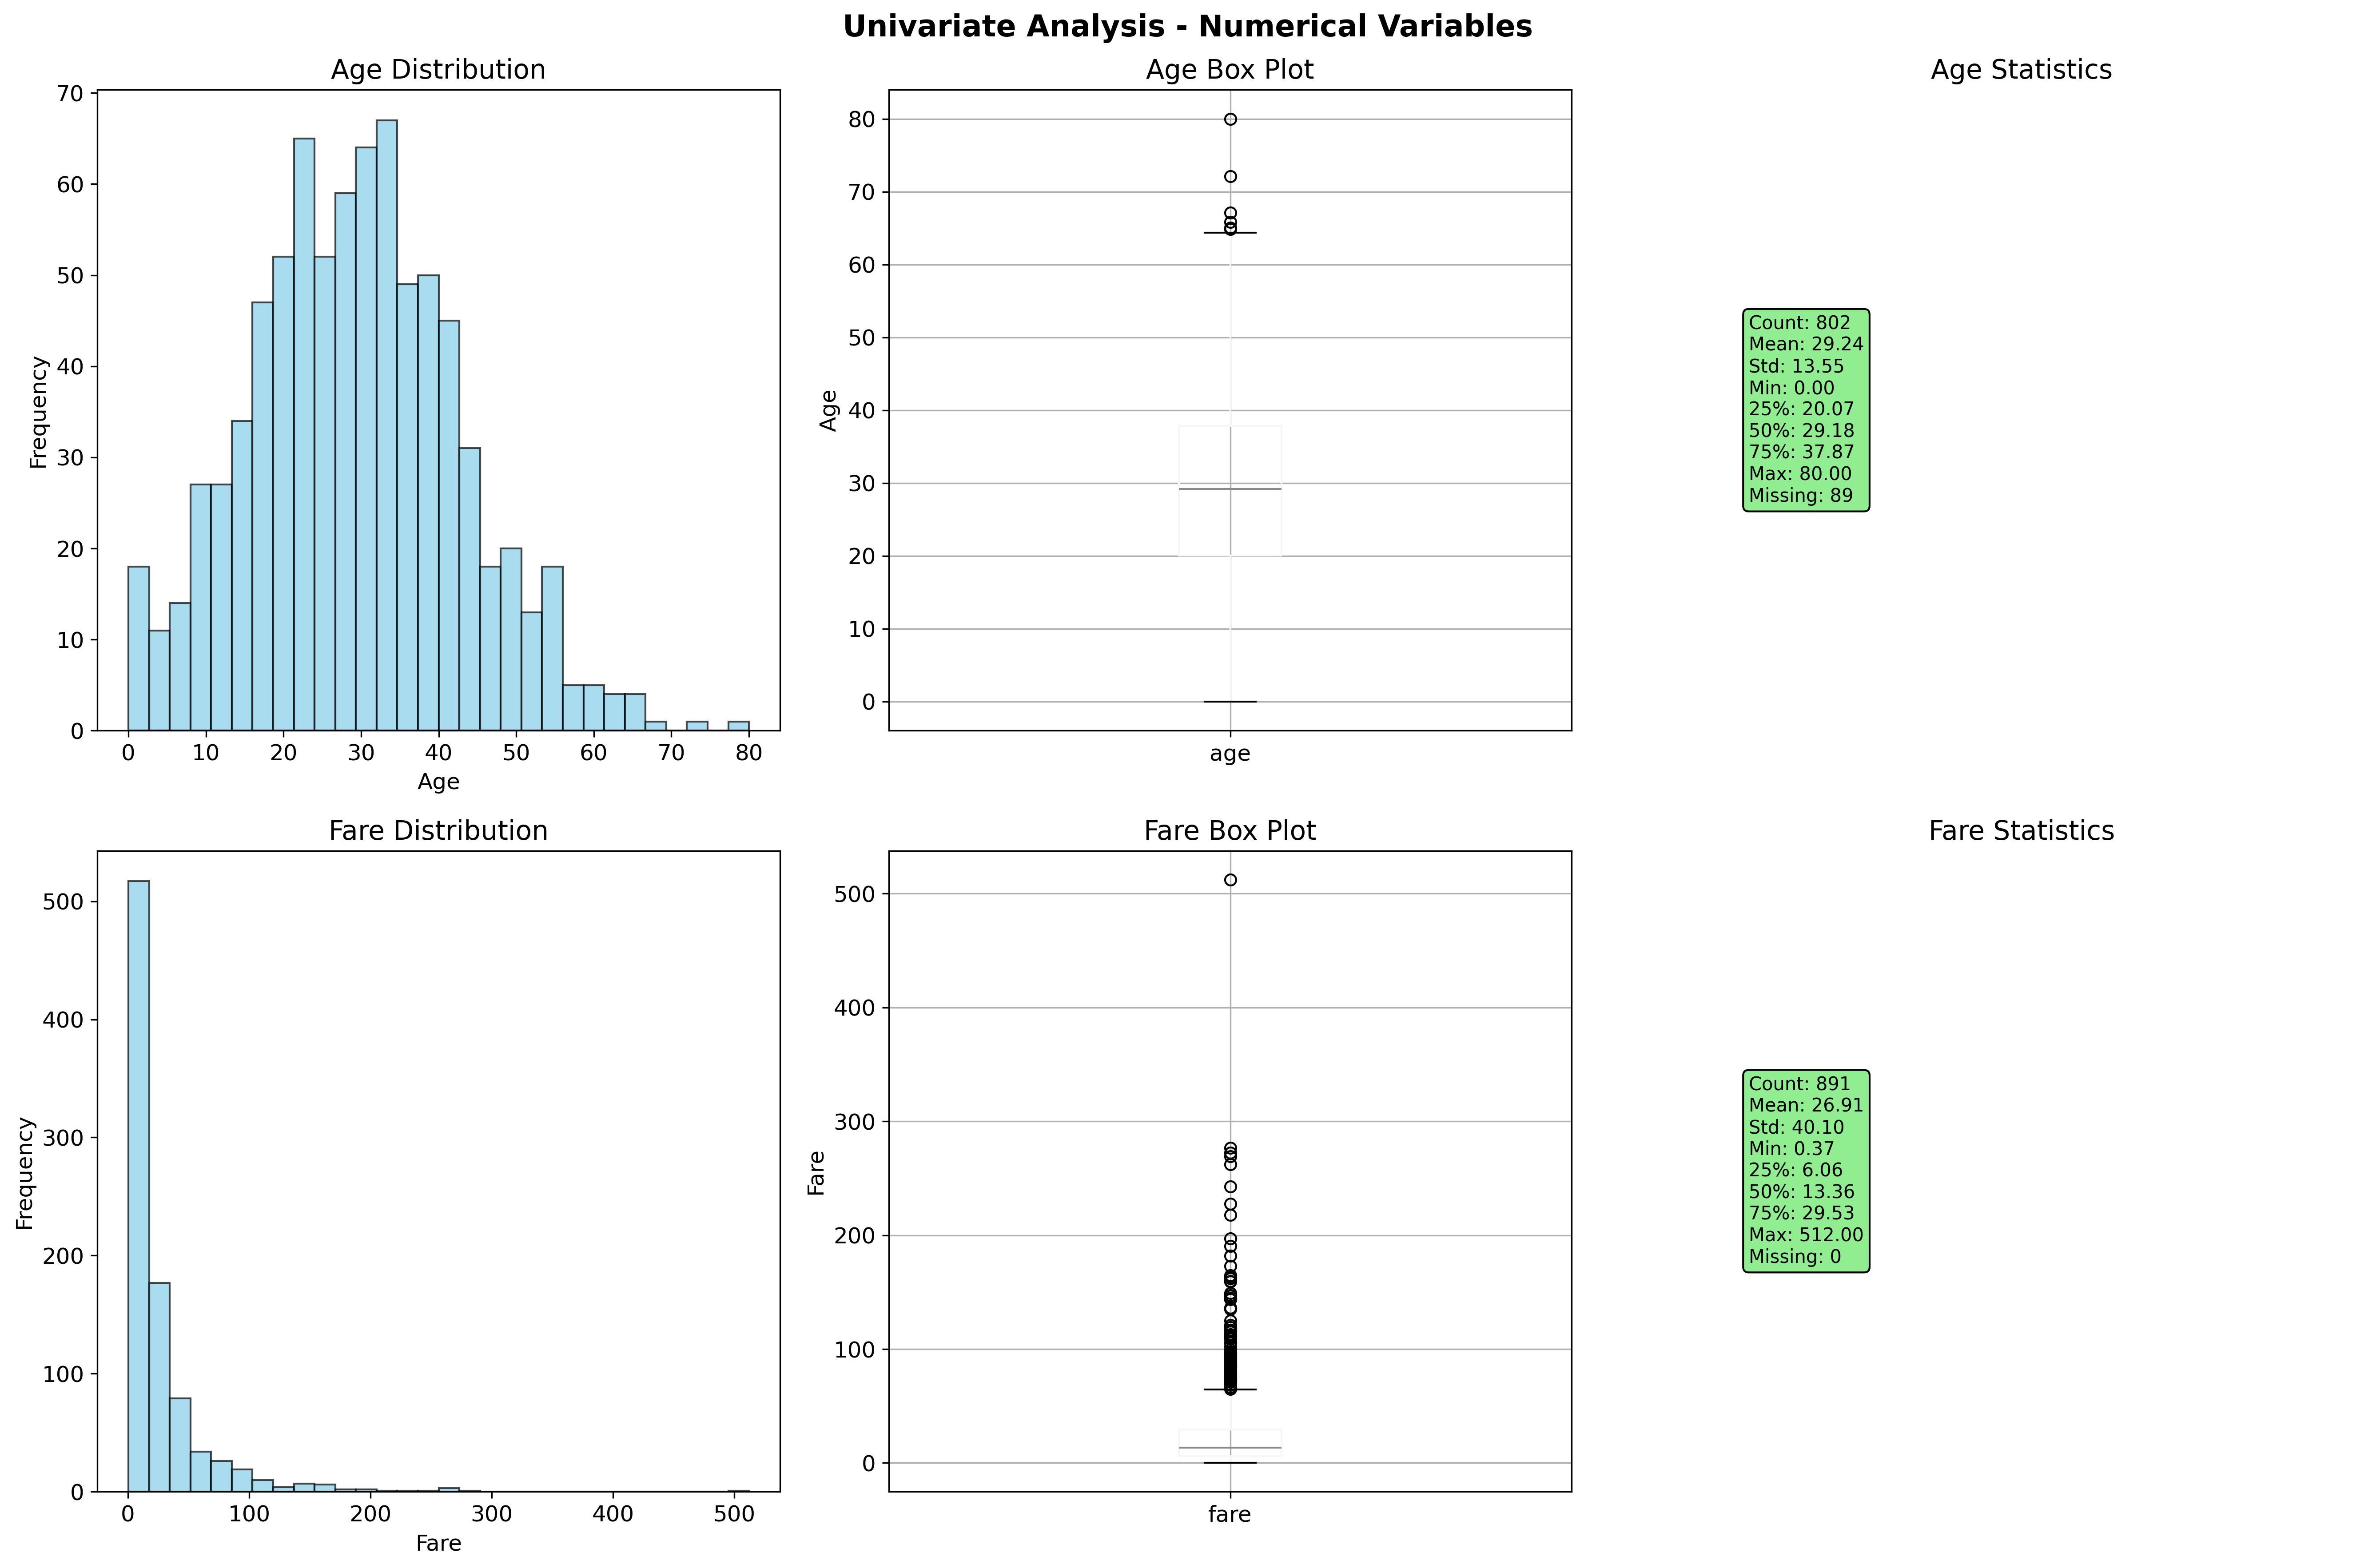
\includegraphics[width=0.9\textwidth]{../figures/02_univariate_numerical.png}
\end{center}

\vspace{0.1cm}
\begin{alertblock}{Key Observations}
\textbf{Age:} Right-skewed, missing values; \textbf{Fare:} Heavy right tail, potential outliers
\end{alertblock}
\end{frame}

\begin{frame}{Statistical Measures for Numerical Data}
\begin{columns}[t]
\begin{column}{0.48\textwidth}
\begin{block}{Central Tendency}
For variable $X = \{x_1, x_2, \ldots, x_n\}$:

\textbf{Mean (Arithmetic):}
$$\bar{x} = \frac{1}{n}\sum_{i=1}^{n} x_i$$

\textbf{Median:} Middle value when sorted
$$\text{Median} = \begin{cases}
x_{(n+1)/2} & \text{if } n \text{ odd} \\
\frac{x_{n/2} + x_{n/2+1}}{2} & \text{if } n \text{ even}
\end{cases}$$

\textbf{Mode:} Most frequent value
\end{block}
\end{column}

\begin{column}{0.48\textwidth}
\begin{block}{Dispersion Measures}
\textbf{Variance:}
$$\sigma^2 = \frac{1}{n-1}\sum_{i=1}^{n}(x_i - \bar{x})^2$$

\textbf{Standard Deviation:}
$$\sigma = \sqrt{\sigma^2}$$

\textbf{Interquartile Range:}
$$\text{IQR} = Q_3 - Q_1$$

\textbf{Range:}
$$\text{Range} = x_{\max} - x_{\min}$$
\end{block}
\end{column}
\end{columns}

\vspace{0.1cm}
\begin{tipblock}{Practical Guidelines}
\textbf{Skewed data:} Use median \& IQR; \textbf{Normal data:} Use mean \& standard deviation
\end{tipblock}
\end{frame}

\begin{frame}{Univariate Analysis - Categorical Variables}
\begin{center}
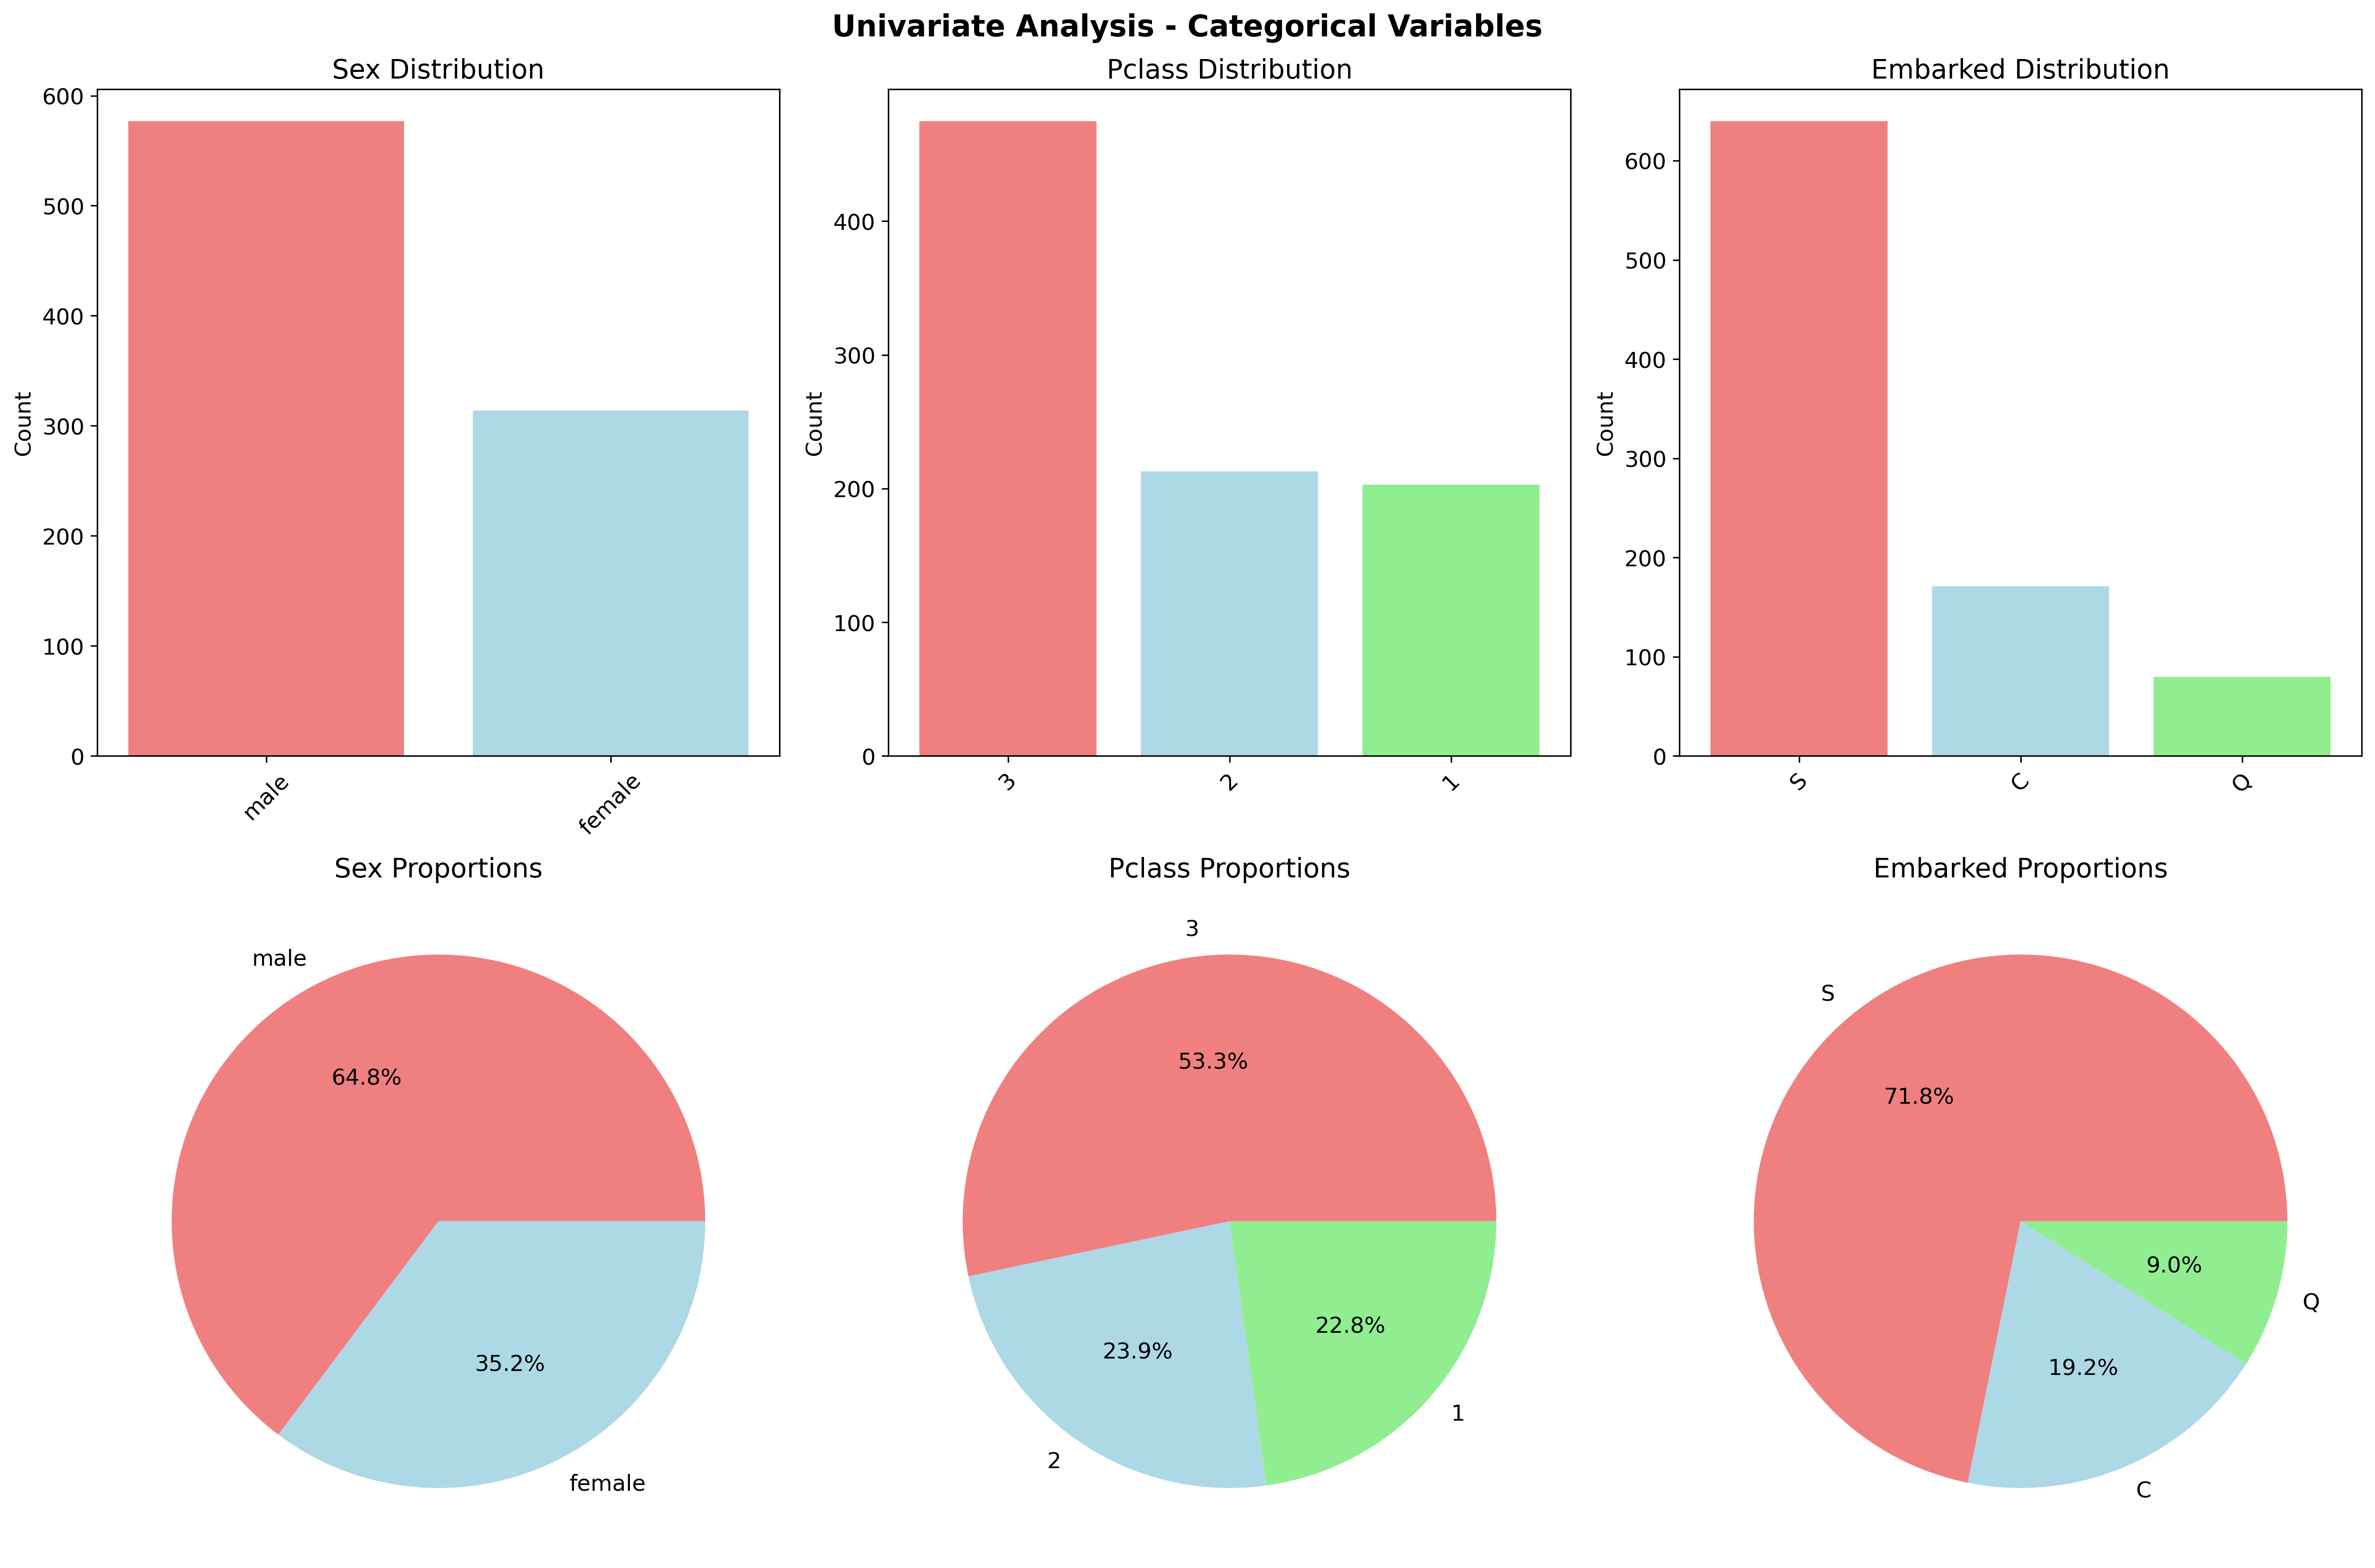
\includegraphics[width=0.9\textwidth]{../figures/03_univariate_categorical.png}
\end{center}

\vspace{0.1cm}
\begin{alertblock}{Key Insights}
\textbf{Gender imbalance:} 65\% male passengers; \textbf{Class distribution:} 55\% third class; \textbf{Embarkation:} 72\% from Southampton
\end{alertblock}
\end{frame}

\begin{frame}{Statistical Measures for Categorical Data}
\begin{columns}[t]
\begin{column}{0.48\textwidth}
\begin{block}{Frequency Analysis}
For categorical variable $C$ with categories $\{c_1, c_2, \ldots, c_k\}$:

\textbf{Frequency:}
$$f_i = \text{count}(C = c_i)$$

\textbf{Relative Frequency:}
$$p_i = \frac{f_i}{n} \text{ where } \sum_{i=1}^{k} p_i = 1$$

\textbf{Mode:} Category with highest frequency
$$\text{Mode} = \arg\max_{c_i} f_i$$
\end{block}

\vspace{0.1cm}
\begin{methodblock}{Entropy Measure}
Information content:
$$H(C) = -\sum_{i=1}^{k} p_i \log_2(p_i)$$
Higher entropy = more uniform distribution
\end{methodblock}
\end{column}

\begin{column}{0.48\textwidth}
\begin{block}{Visualization Guidelines}
\textbf{Bar Charts:}
\begin{itemize}
\setlength{\itemsep}{1pt}
\item Best for comparing categories
\item Order by frequency for impact
\item Use consistent colors
\end{itemize}

\textbf{Pie Charts:}
\begin{itemize}
\setlength{\itemsep}{1pt}
\item Good for showing proportions
\item Limit to $\leq 5$ categories
\item Start largest slice at 12 o'clock
\end{itemize}
\end{block}

\vspace{0.1cm}
\begin{exampleblock}{Chi-Square Test}
Test for uniform distribution:
$$\chi^2 = \sum_{i=1}^{k} \frac{(O_i - E_i)^2}{E_i}$$
where $O_i$ = observed, $E_i$ = expected
\end{exampleblock}
\end{column}
\end{columns}
\end{frame}

\begin{frame}{Distribution Analysis \& Normality Testing}
\begin{columns}[t]
\begin{column}{0.48\textwidth}
\begin{block}{Common Distributions}
\textbf{Normal Distribution:}
$$f(x) = \frac{1}{\sigma\sqrt{2\pi}} e^{-\frac{(x-\mu)^2}{2\sigma^2}}$$

\textbf{Log-Normal Distribution:}
$$f(x) = \frac{1}{x\sigma\sqrt{2\pi}} e^{-\frac{(\ln x-\mu)^2}{2\sigma^2}}$$

\textbf{Skewness:}
$$\text{Skew} = \frac{E[(X-\mu)^3]}{\sigma^3}$$
\end{block}
\end{column}

\begin{column}{0.48\textwidth}
\begin{block}{Normality Tests}
\textbf{Shapiro-Wilk Test:}
$$W = \frac{(\sum_{i=1}^n a_i x_{(i)})^2}{\sum_{i=1}^n (x_i - \bar{x})^2}$$

\textbf{Kolmogorov-Smirnov Test:}
$$D = \sup_x |F_n(x) - F(x)|$$

\textbf{Anderson-Darling Test:}
More sensitive to tail deviations
\end{block}
\end{column}
\end{columns}

\vspace{0.1cm}
\begin{alertblock}{Decision Rule}
If $p < 0.05$: Reject normality assumption; Consider transformations (log, square root, Box-Cox)
\end{alertblock}
\end{frame}

% ========================================
% Section: Bivariate Analysis
% ========================================

\section{Bivariate Analysis}

\begin{frame}{Correlation Analysis}
\begin{center}
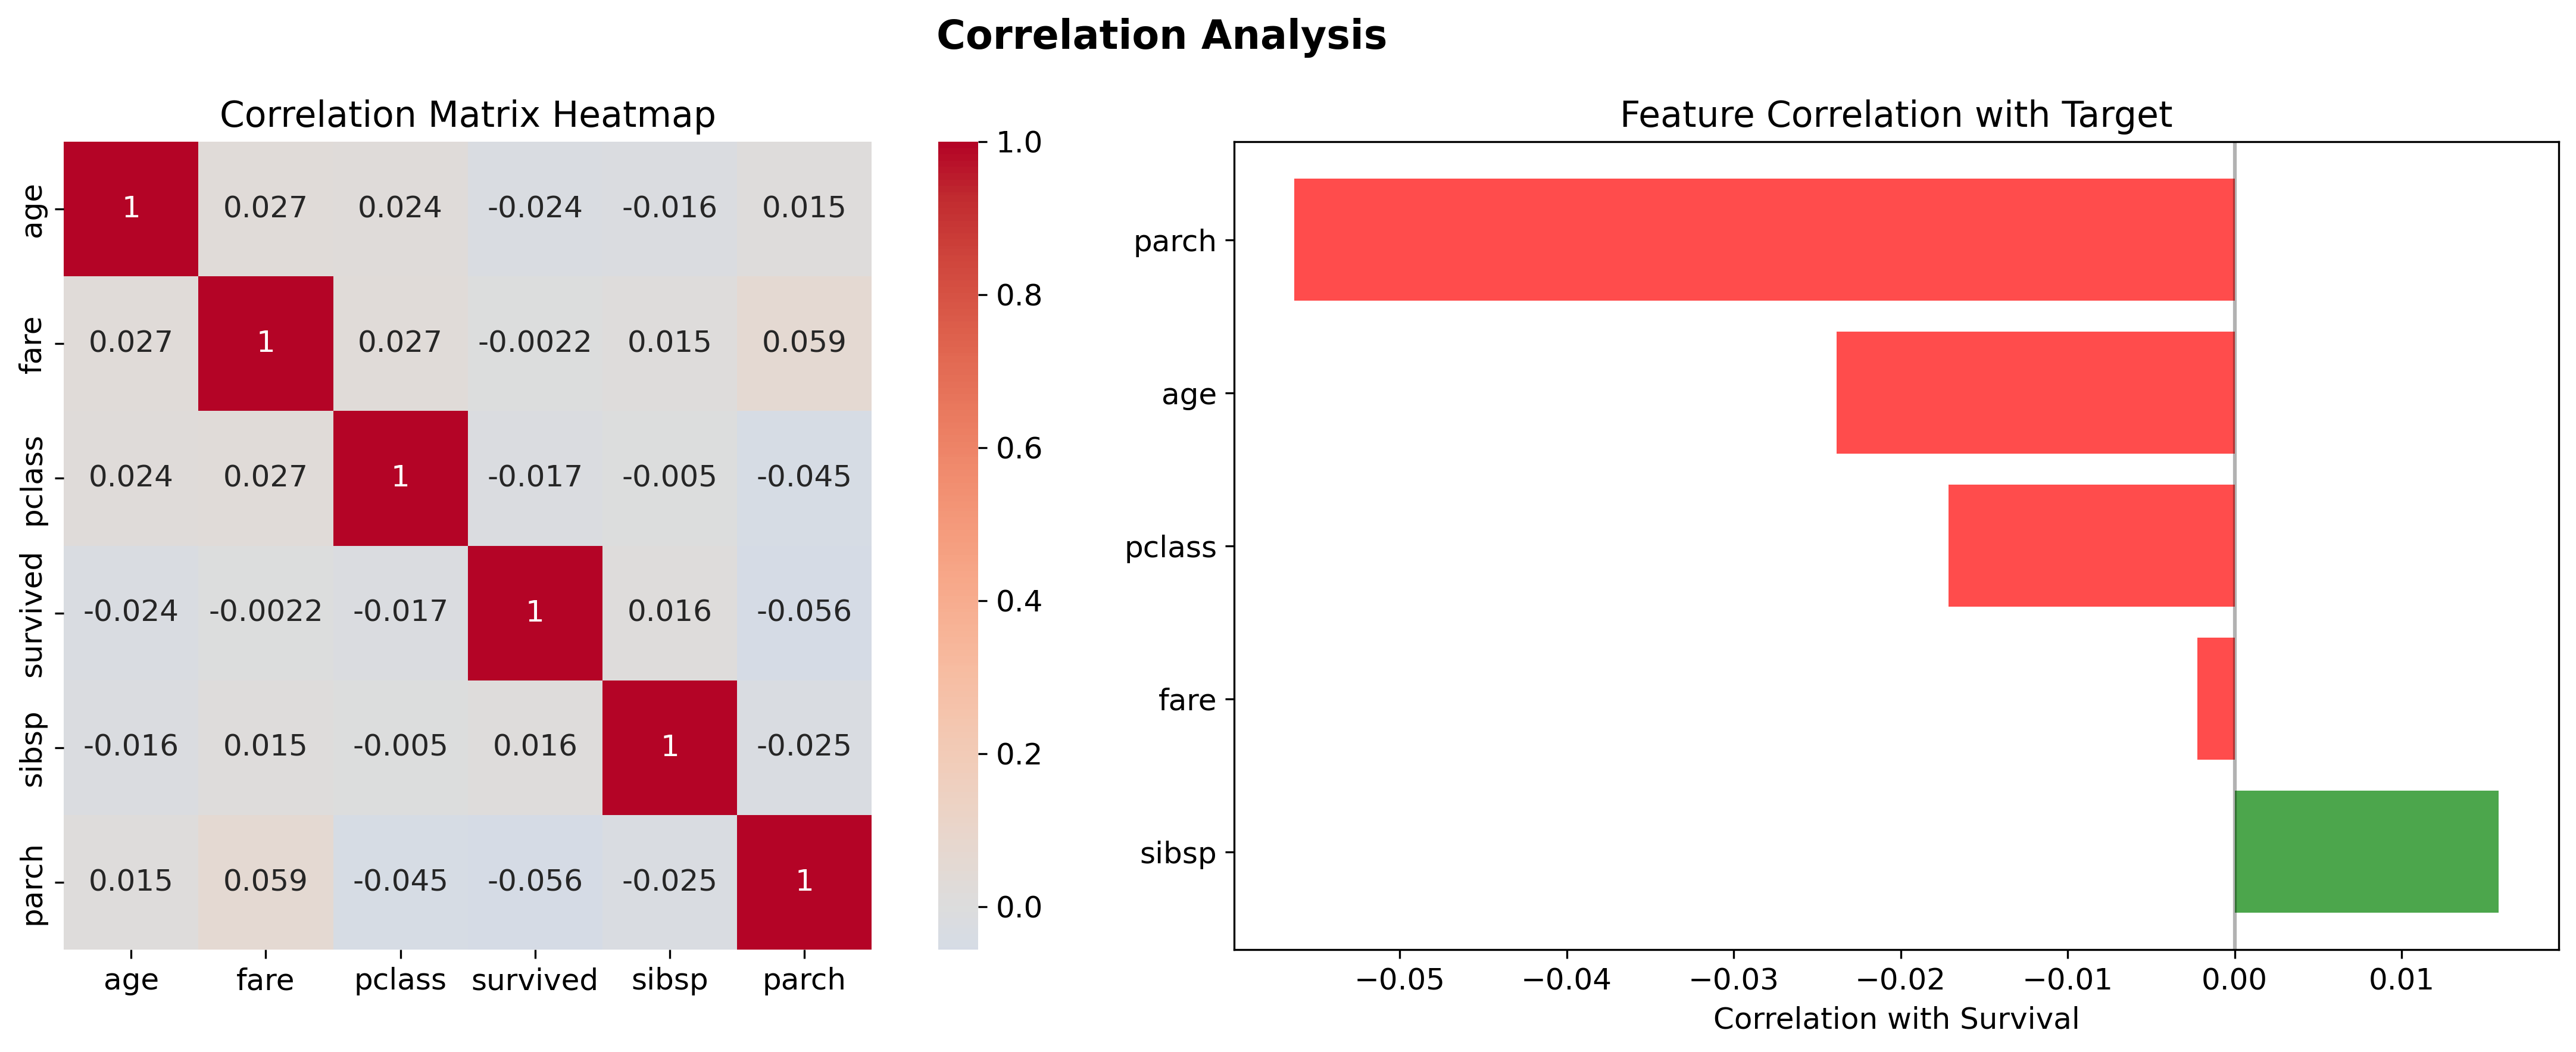
\includegraphics[width=0.9\textwidth]{../figures/04_correlation_analysis.png}
\end{center}

\vspace{0.1cm}
\begin{alertblock}{Correlation Insights}
\textbf{Strong correlations:} Fare-Survival (0.26), Age-Survival (-0.07); \textbf{Weak correlations:} SibSp-Parch (0.41)
\end{alertblock}
\end{frame}

\begin{frame}{Correlation Coefficients \& Interpretation}
\begin{columns}[t]
\begin{column}{0.48\textwidth}
\begin{block}{Pearson Correlation}
For linear relationships:
$$r = \frac{\sum_{i=1}^{n}(x_i - \bar{x})(y_i - \bar{y})}{\sqrt{\sum_{i=1}^{n}(x_i - \bar{x})^2 \sum_{i=1}^{n}(y_i - \bar{y})^2}}$$

\textbf{Range:} $r \in [-1, 1]$
\begin{itemize}
\setlength{\itemsep}{1pt}
\item $r = 1$: Perfect positive correlation
\item $r = 0$: No linear correlation
\item $r = -1$: Perfect negative correlation
\end{itemize}
\end{block}

\vspace{0.1cm}
\begin{methodblock}{Significance Test}
$$t = r\sqrt{\frac{n-2}{1-r^2}} \sim t_{n-2}$$
\end{methodblock}
\end{column}

\begin{column}{0.48\textwidth}
\begin{block}{Non-Linear Correlations}
\textbf{Spearman Rank Correlation:}
$$\rho = 1 - \frac{6\sum d_i^2}{n(n^2-1)}$$
where $d_i$ = rank difference

\textbf{Kendall's Tau:}
$$\tau = \frac{n_c - n_d}{\frac{1}{2}n(n-1)}$$
where $n_c$ = concordant pairs, $n_d$ = discordant pairs
\end{block}

\vspace{0.1cm}
\begin{exampleblock}{Interpretation Guide}
\begin{itemize}
\setlength{\itemsep}{1pt}
\item $|r| < 0.3$: Weak relationship
\item $0.3 \leq |r| < 0.7$: Moderate relationship
\item $|r| \geq 0.7$: Strong relationship
\end{itemize}
\end{exampleblock}
\end{column}
\end{columns}

\begin{alertblock}{Remember}
\textbf{Correlation $\neq$ Causation!} Always investigate the underlying mechanisms.
\end{alertblock}
\end{frame}

\begin{frame}{Bivariate Analysis - Feature Relationships}
\begin{center}
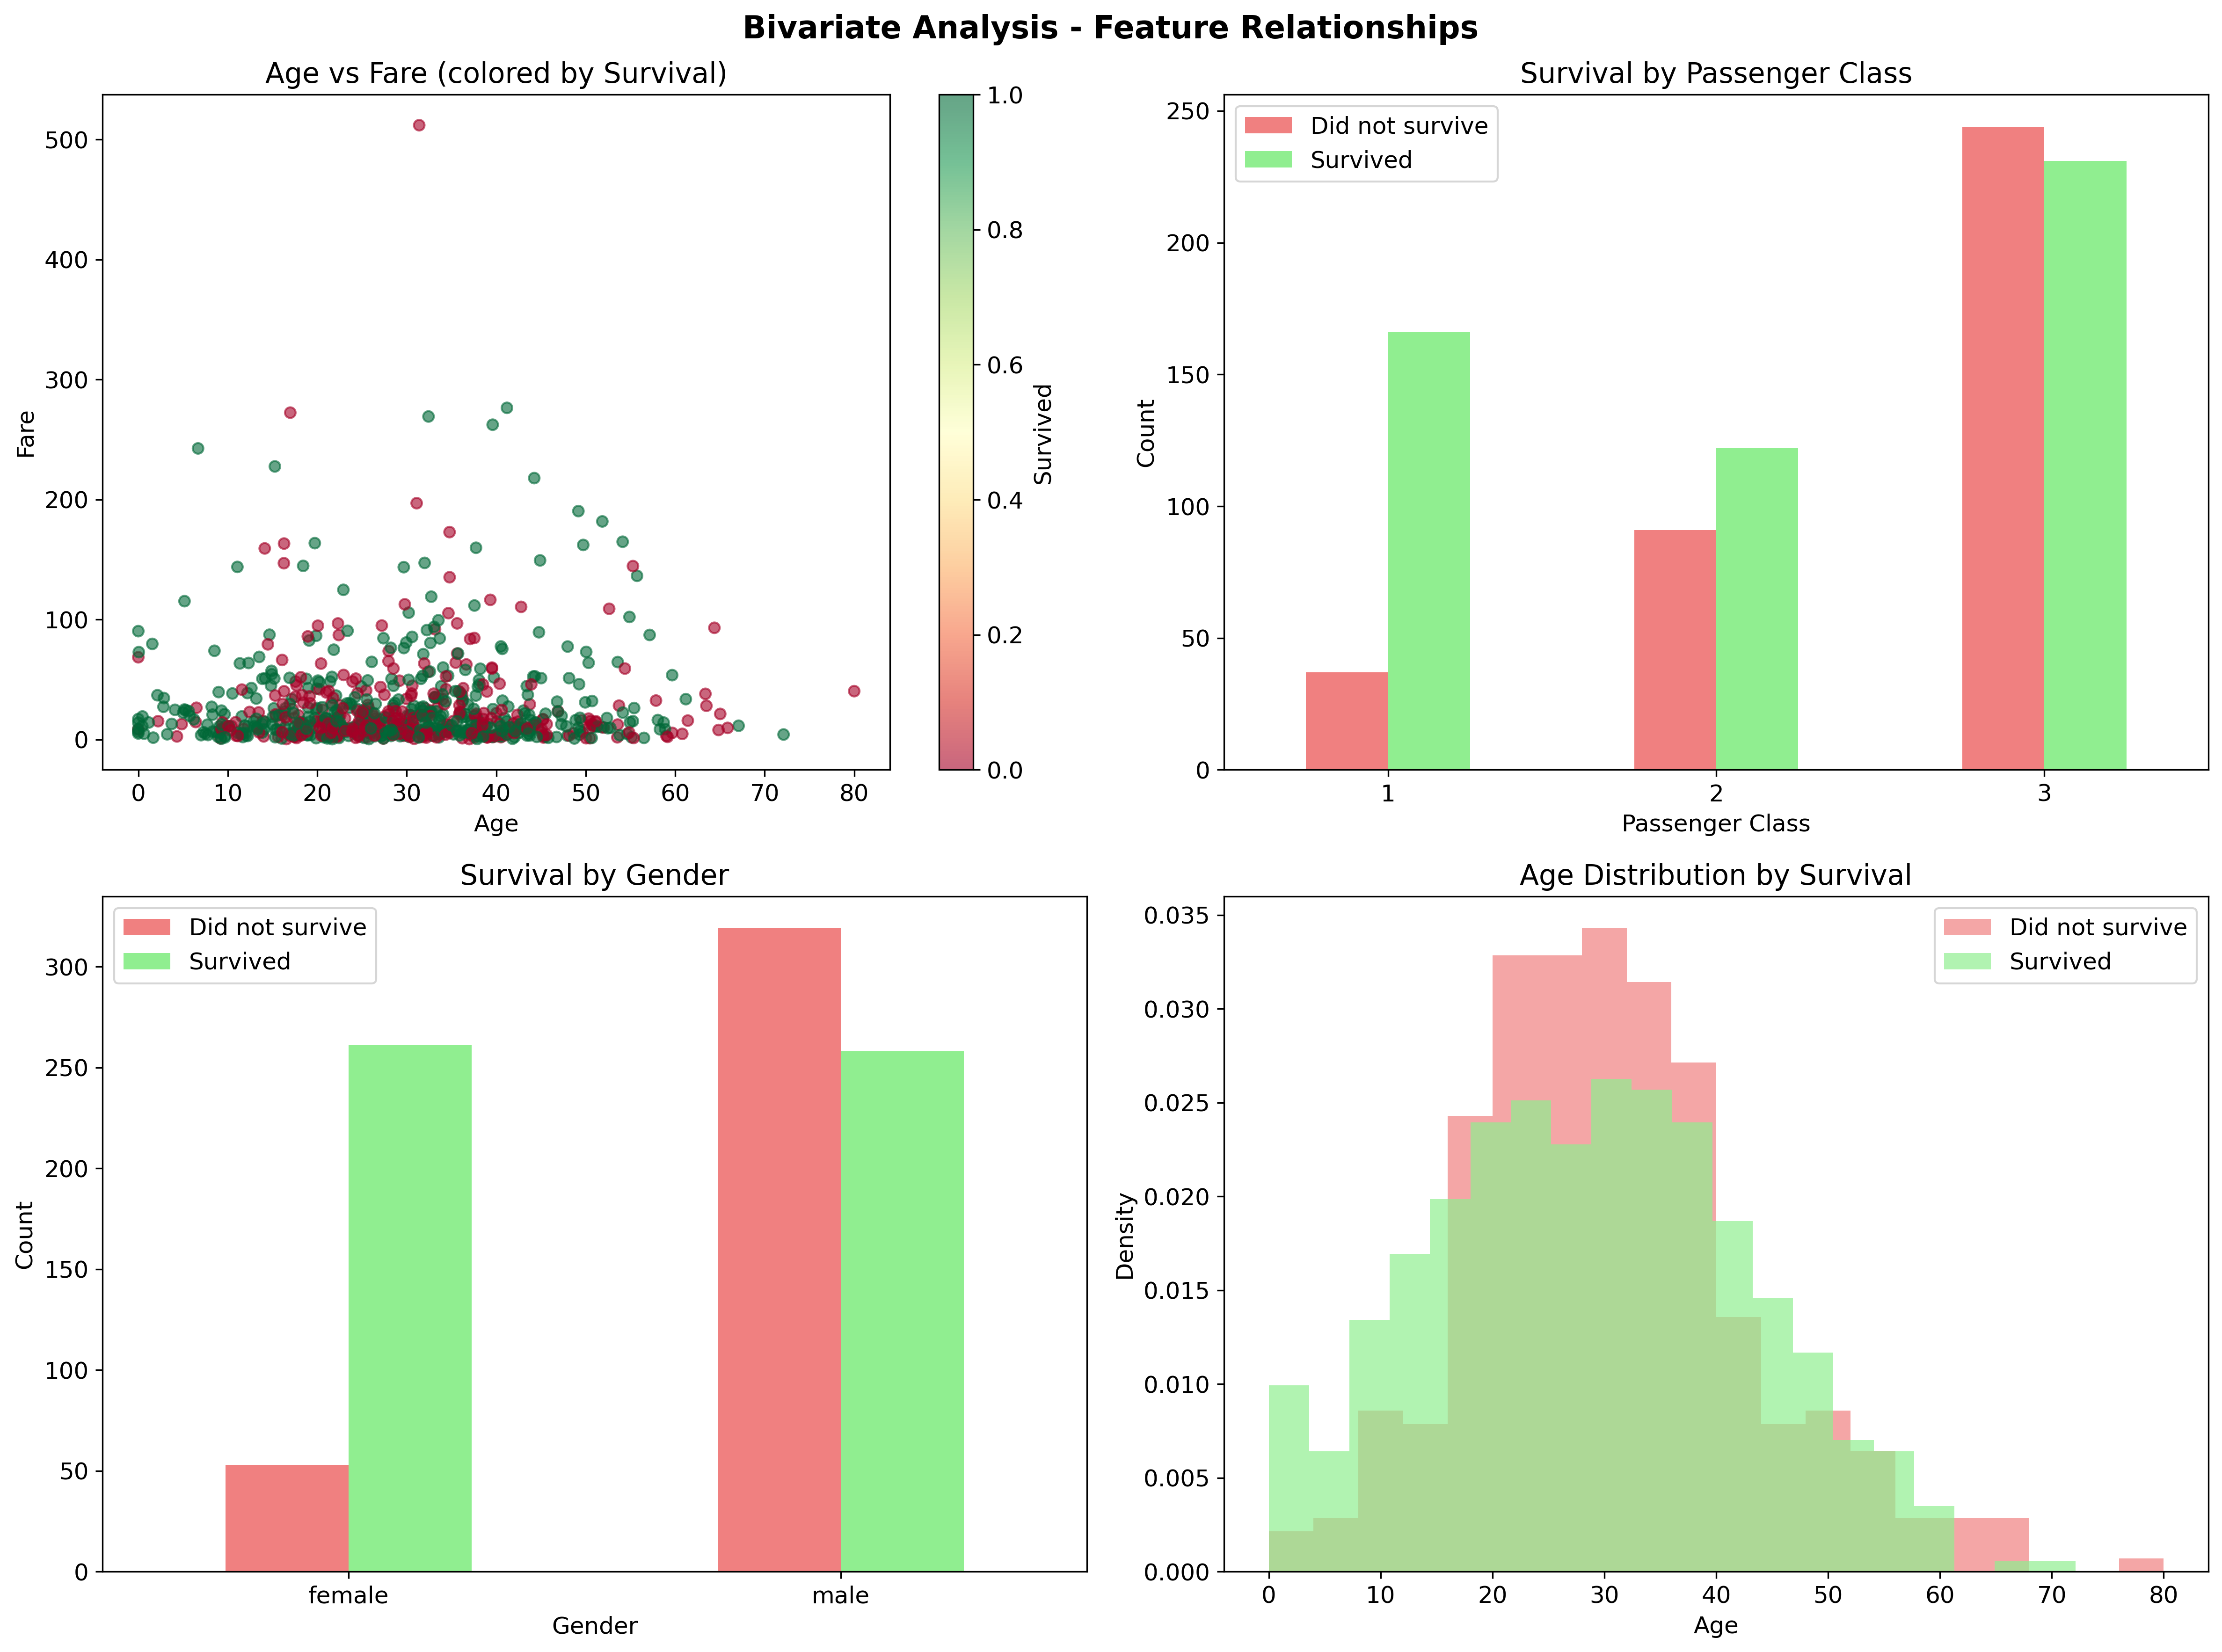
\includegraphics[width=0.9\textwidth]{../figures/10_bivariate_analysis.png}
\end{center}

\vspace{0.1cm}
\begin{alertblock}{Key Patterns}
\textbf{Gender effect:} Women had 74\% survival rate vs men 19\%; \textbf{Class effect:} 1st class 63\% vs 3rd class 24\%
\end{alertblock}
\end{frame}

\begin{frame}{Cross-Tabulation \& Contingency Tables}
\begin{columns}[t]
\begin{column}{0.48\textwidth}
\begin{block}{Contingency Table}
For categorical variables $A$ and $B$:

\begin{center}
\small
\begin{tabular}{|c|c|c|c|}
\hline
 & $B_1$ & $B_2$ & Total \\
\hline
$A_1$ & $n_{11}$ & $n_{12}$ & $n_{1.}$ \\
$A_2$ & $n_{21}$ & $n_{22}$ & $n_{2.}$ \\
\hline
Total & $n_{.1}$ & $n_{.2}$ & $n$ \\
\hline
\end{tabular}
\end{center}

\textbf{Joint Probability:}
$$P(A_i, B_j) = \frac{n_{ij}}{n}$$

\textbf{Marginal Probability:}
$$P(A_i) = \frac{n_{i.}}{n}, \quad P(B_j) = \frac{n_{.j}}{n}$$
\end{block}
\end{column}

\begin{column}{0.48\textwidth}
\begin{block}{Independence Test}
\textbf{Chi-Square Test:}
$$\chi^2 = \sum_{i,j} \frac{(O_{ij} - E_{ij})^2}{E_{ij}}$$

where $E_{ij} = \frac{n_{i.} \times n_{.j}}{n}$

\textbf{Degrees of freedom:}
$$df = (r-1)(c-1)$$

\textbf{Cramér's V (Effect Size):}
$$V = \sqrt{\frac{\chi^2}{n \times \min(r-1, c-1)}}$$
\end{block}

\vspace{0.1cm}
\begin{tipblock}{Interpretation}
$V \in [0,1]$: 0 = no association, 1 = perfect association
\end{tipblock}
\end{column}
\end{columns}
\end{frame}

% ========================================
% Section: Missing Data Analysis
% ========================================

\section{Missing Data Handling}

\begin{frame}{Missing Data Analysis}
\begin{center}
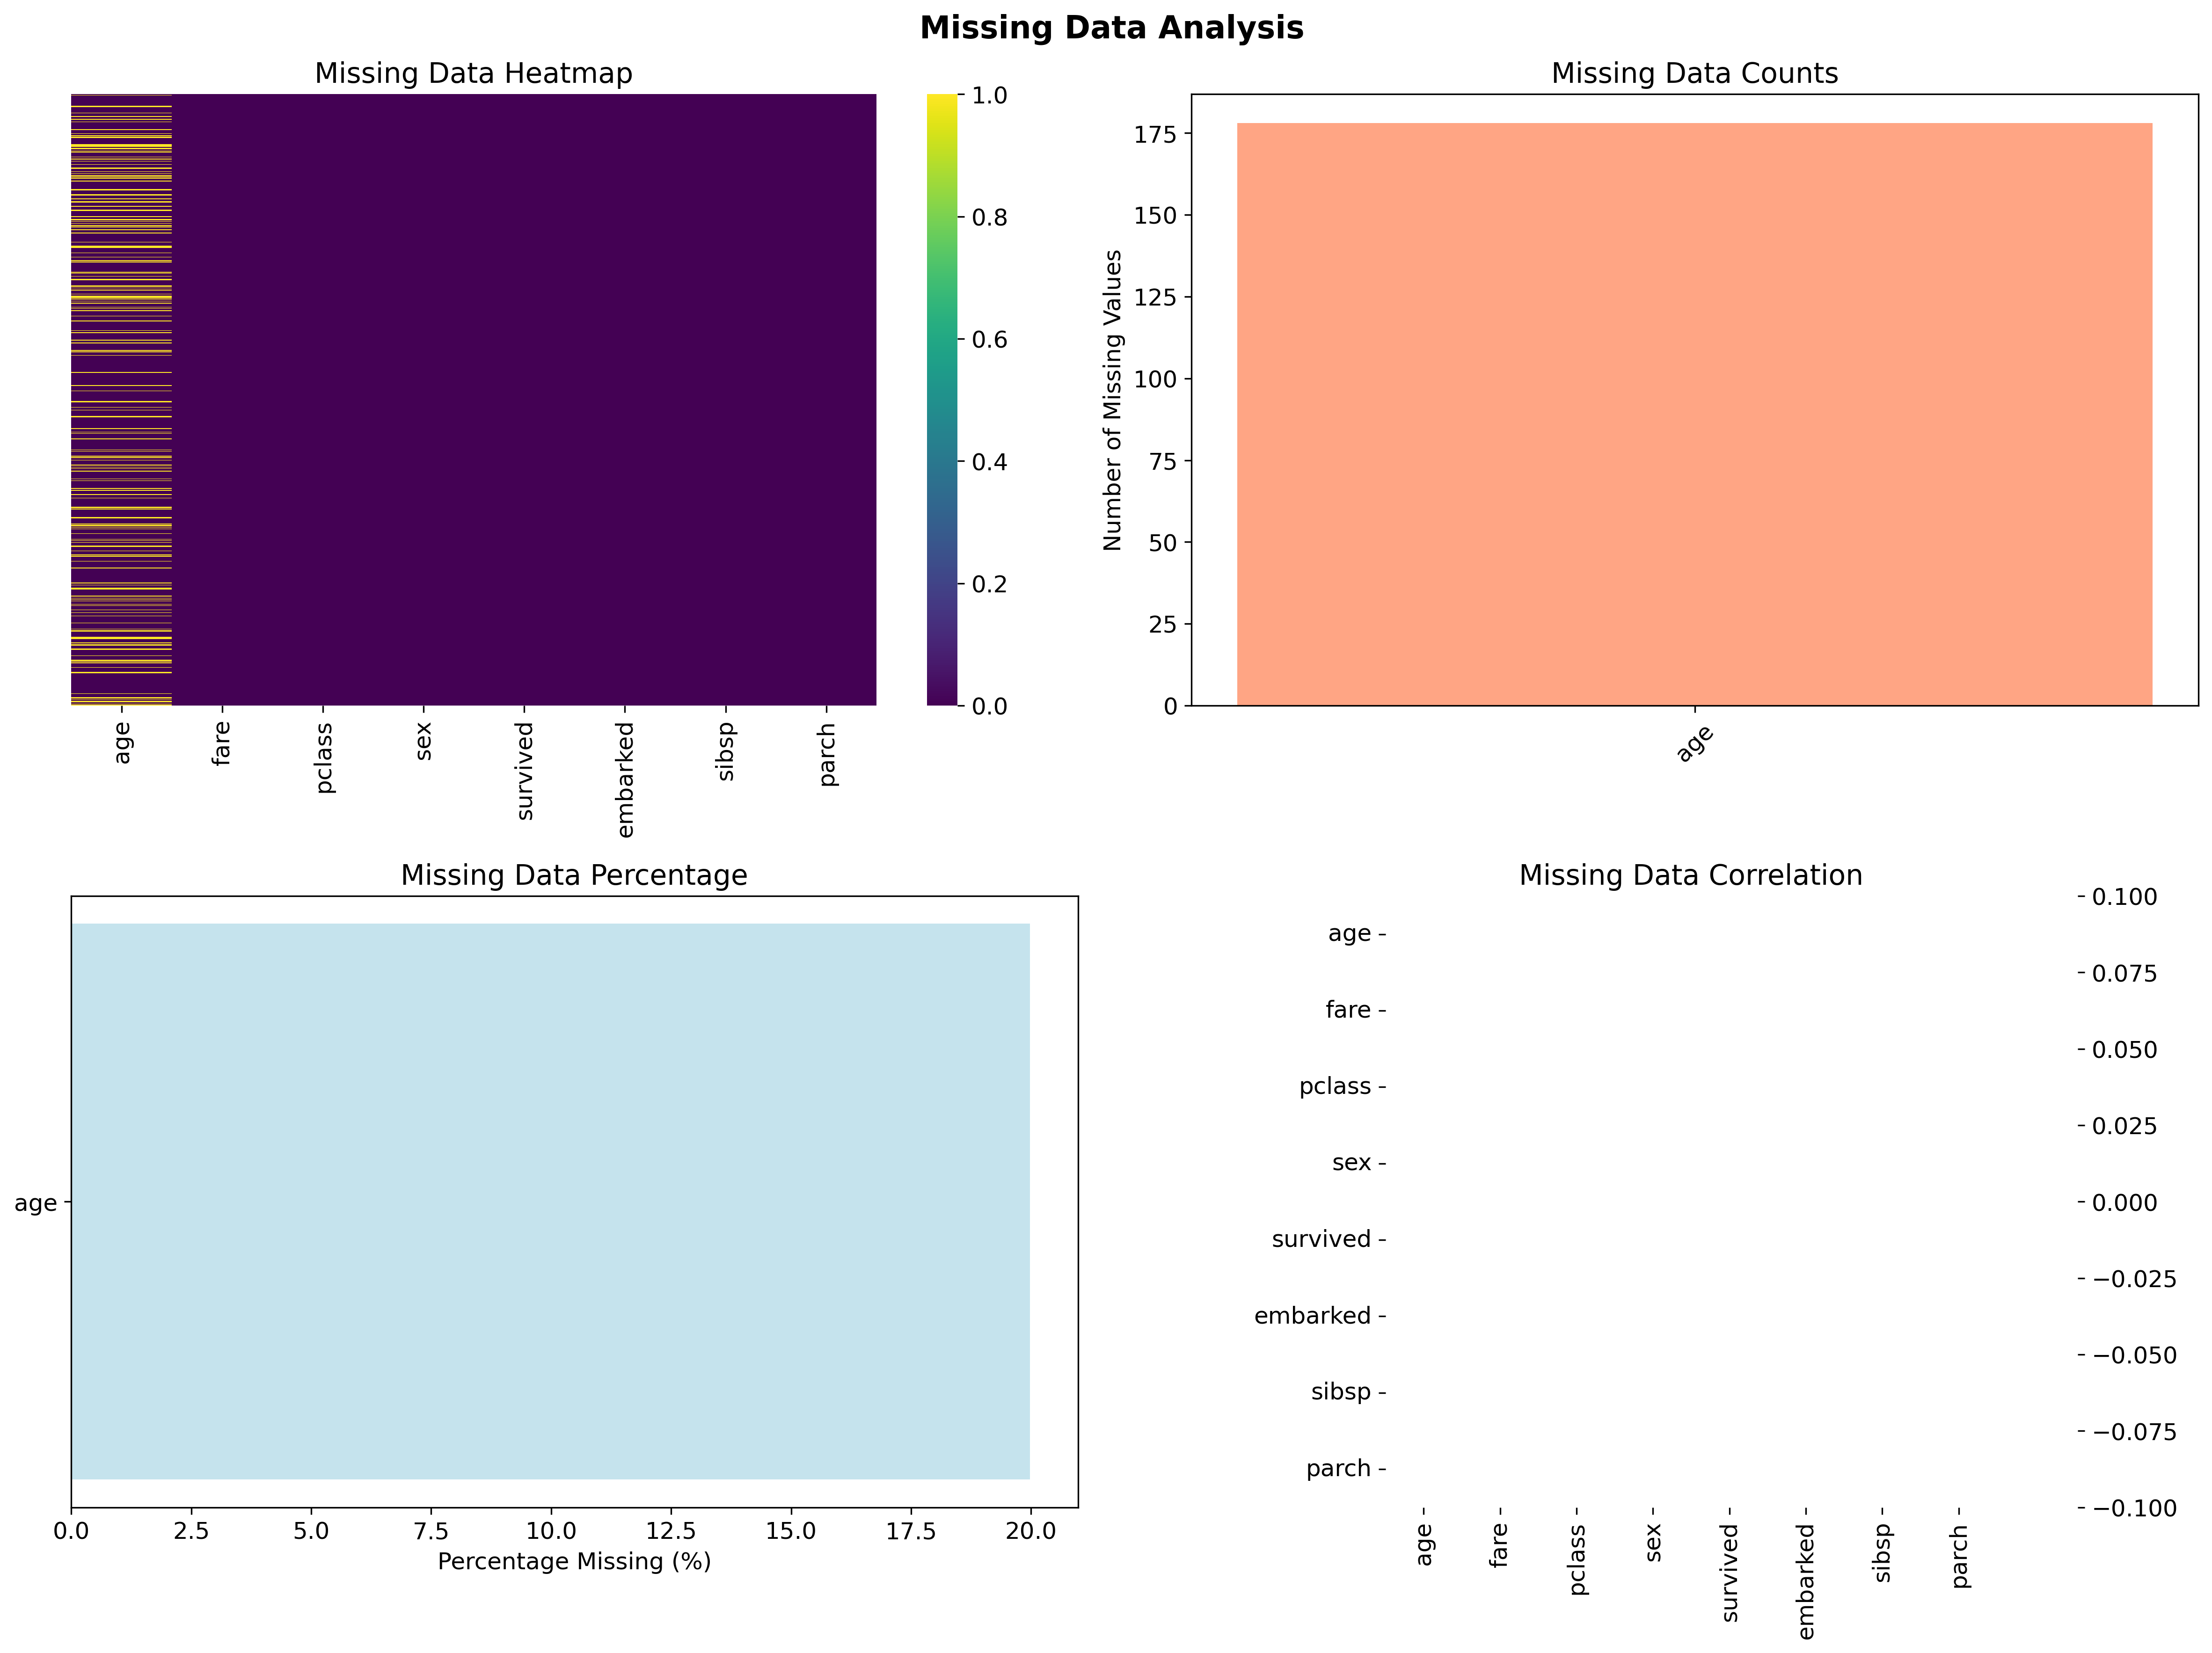
\includegraphics[width=0.9\textwidth]{../figures/05_missing_data_analysis.png}
\end{center}

\vspace{0.1cm}
\begin{alertblock}{Missing Data Impact}
\textbf{Age:} 20\% missing values; \textbf{Pattern:} May not be random - could be related to passenger class or survival
\end{alertblock}
\end{frame}

\begin{frame}{Types of Missing Data}
\begin{columns}[t]
\begin{column}{0.48\textwidth}
\begin{block}{MCAR: Missing Completely at Random}
\textbf{Definition:} Missing data is independent of both observed and unobserved data.

\textbf{Mathematical condition:}
$$P(\text{Missing} | X, Y) = P(\text{Missing})$$

\textbf{Example:} Survey responses lost due to mail delivery issues.

\textbf{Implication:} Can use any imputation method without bias.
\end{block}

\vspace{0.1cm}
\begin{methodblock}{Test for MCAR}
\textbf{Little's MCAR Test:}
Tests null hypothesis that data is MCAR using EM algorithm.
\end{methodblock}
\end{column}

\begin{column}{0.48\textwidth}
\begin{block}{MAR: Missing at Random}
\textbf{Definition:} Missing data depends on observed data, but not on unobserved data.

\textbf{Mathematical condition:}
$$P(\text{Missing} | X, Y) = P(\text{Missing} | X)$$

\textbf{Example:} Older passengers more likely to have missing age data.

\textbf{MNAR: Missing Not at Random}
Missing data depends on unobserved data.

\textbf{Example:} High-income individuals not reporting income.
\end{block}

\vspace{0.1cm}
\begin{alertblock}{Handling Strategy}
\textbf{MAR:} Multiple imputation; \textbf{MNAR:} Domain expertise required
\end{alertblock}
\end{column}
\end{columns}
\end{frame}

\begin{frame}{Imputation Strategies}
\begin{columns}[t]
\begin{column}{0.48\textwidth}
\begin{block}{Simple Imputation}
\textbf{Mean/Mode Imputation:}
$$x_{\text{missing}} = \bar{x} \text{ or Mode}(x)$$

\textbf{Median Imputation:}
$$x_{\text{missing}} = \text{Median}(x)$$

\textbf{Forward/Backward Fill:}
For time series data

\textbf{Constant Value:}
Domain-specific constant (e.g., 0, -1)
\end{block}

\vspace{0.1cm}
\begin{alertblock}{Limitations}
Simple methods reduce variance and can introduce bias
\end{alertblock}
\end{column}

\begin{column}{0.48\textwidth}
\begin{block}{Advanced Imputation}
\textbf{KNN Imputation:}
$$x_{\text{missing}} = \frac{1}{k}\sum_{i \in \text{k-nearest}} x_i$$

\textbf{Multiple Imputation:}
Creates multiple complete datasets, analyzes each, pools results.

\textbf{Model-based:}
- Linear regression
- Random Forest
- Deep learning approaches
\end{block}

\vspace{0.1cm}
\begin{exampleblock}{Best Practice}
\textbf{Always analyze missing data pattern before choosing imputation method}
\end{exampleblock}
\end{column}
\end{columns}
\end{frame}

% ========================================
% Section: Outlier Detection
% ========================================

\section{Outlier Detection}

\begin{frame}{Outlier Detection Methods}
\begin{center}
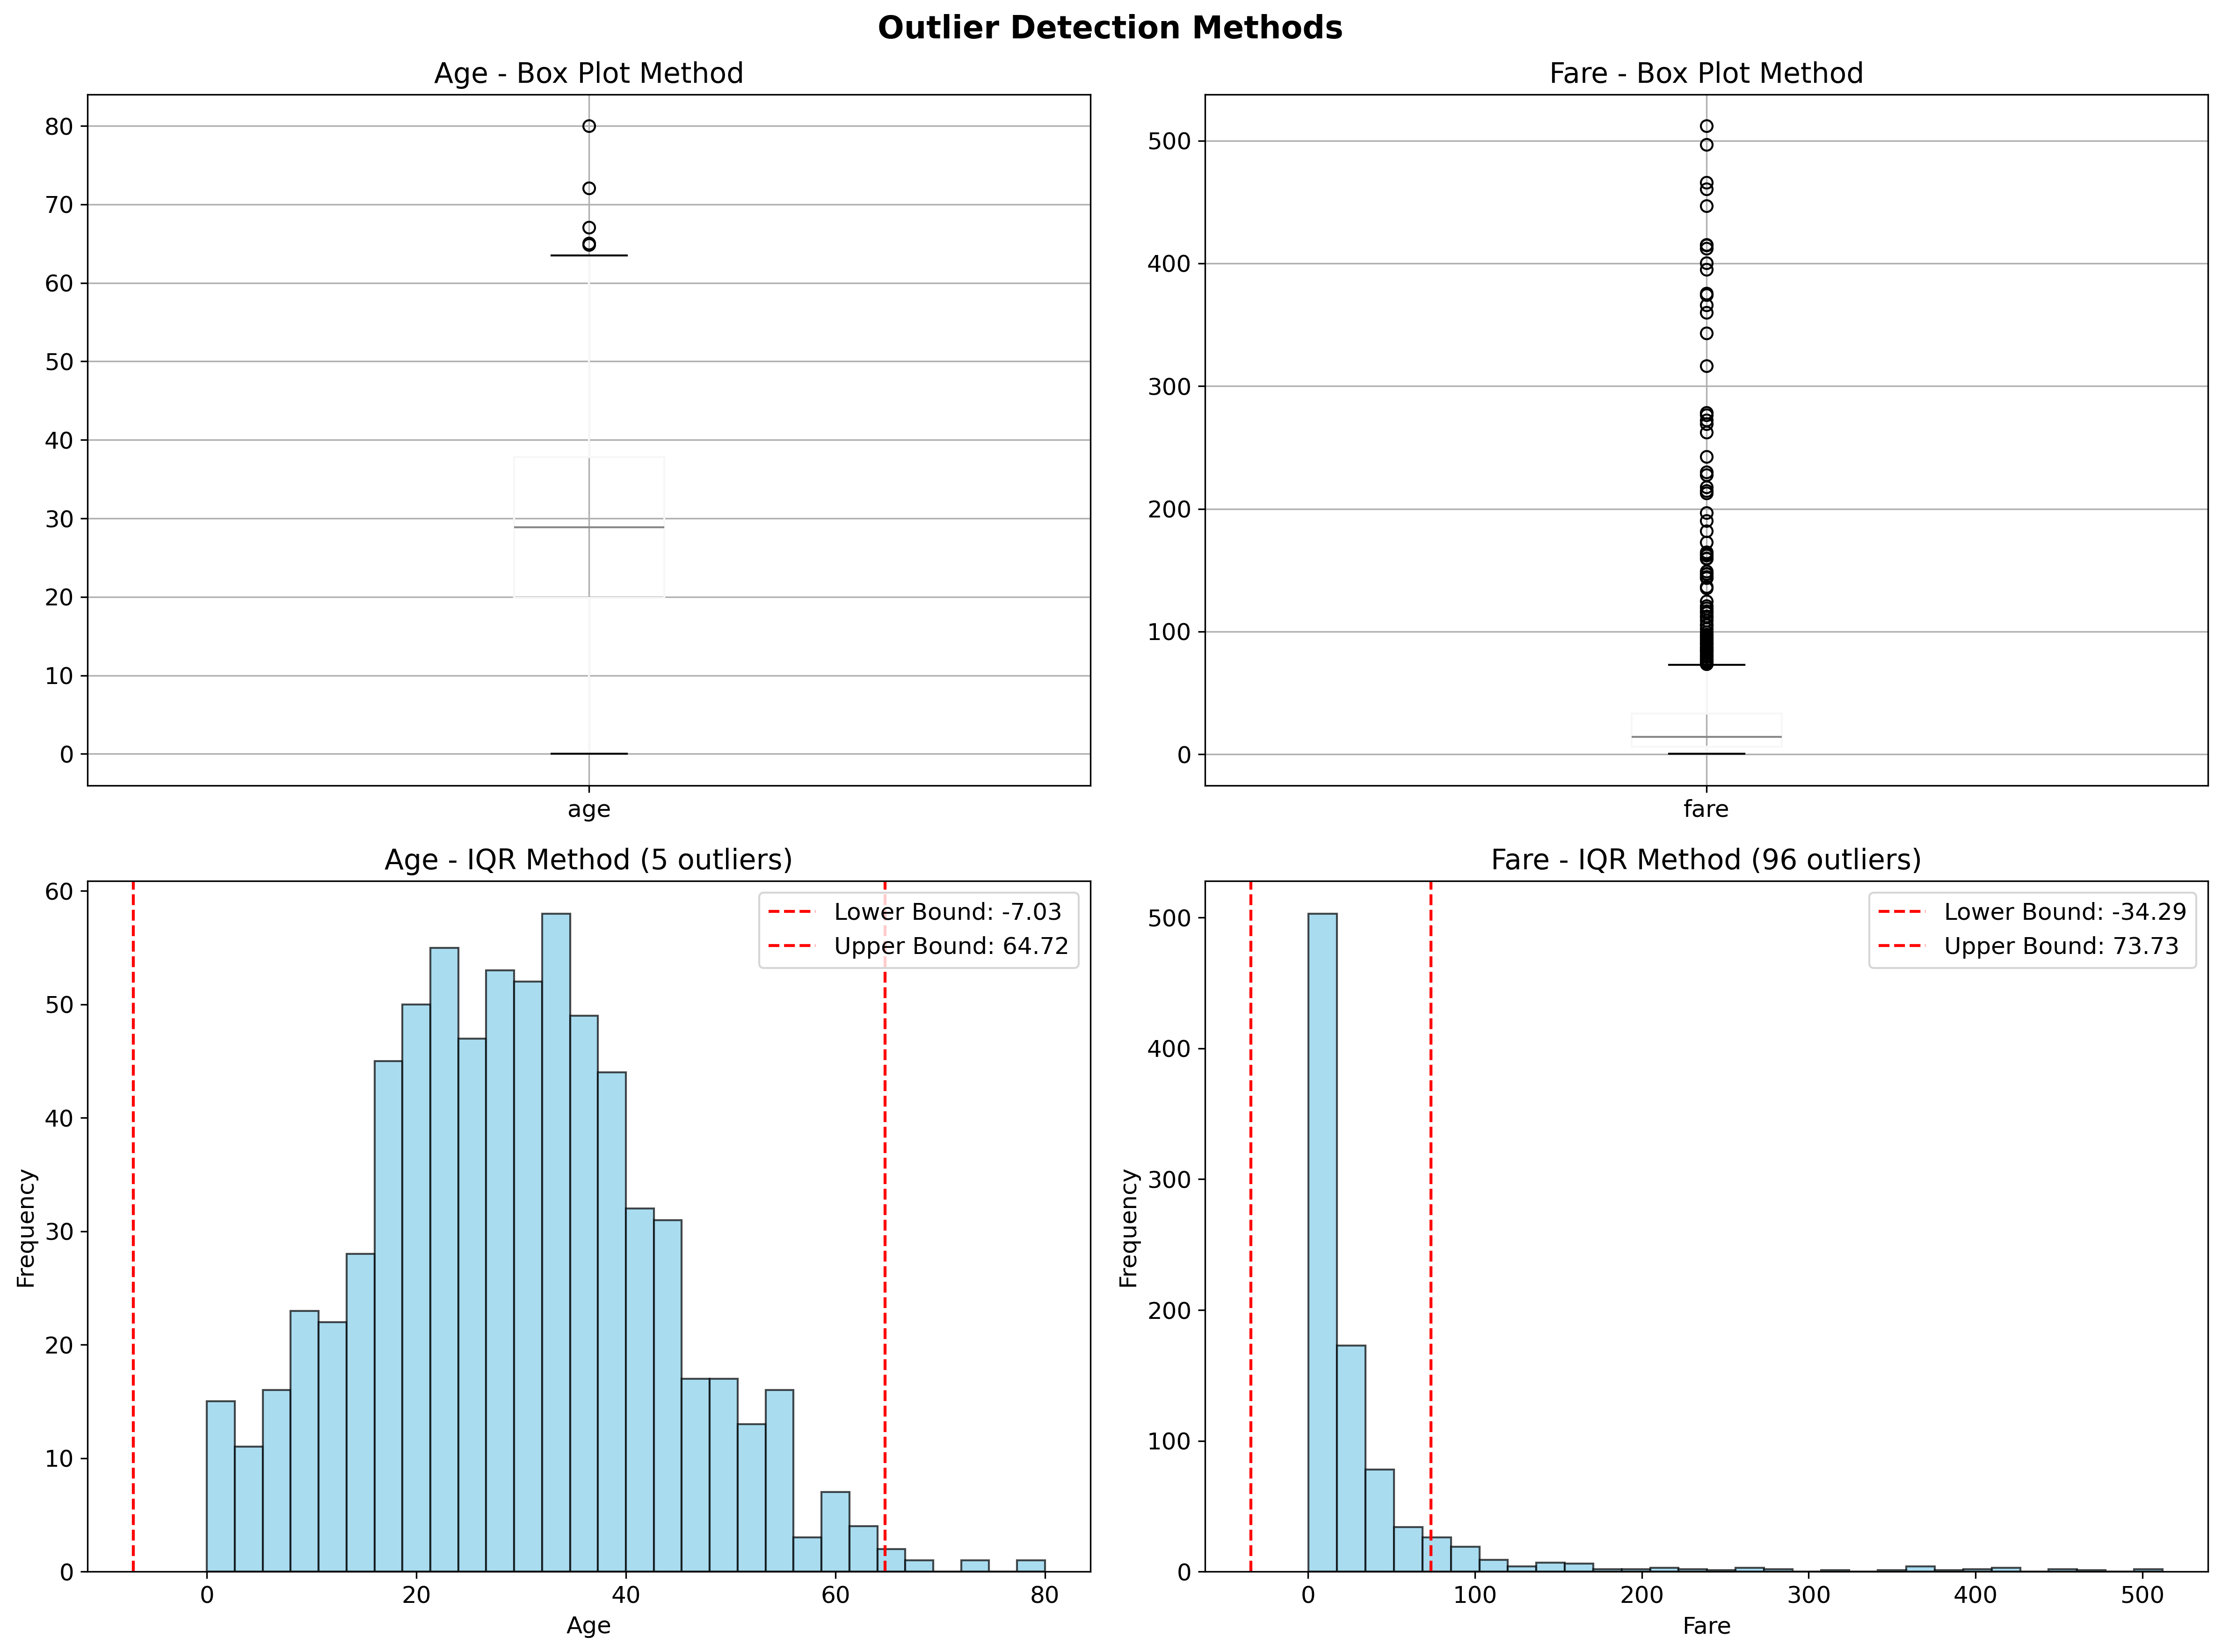
\includegraphics[width=0.9\textwidth]{../figures/06_outlier_detection.png}
\end{center}

\vspace{0.1cm}
\begin{alertblock}{Outlier Findings}
\textbf{Fare:} 20 outliers detected using IQR method; \textbf{Age:} Few extreme values at high ages
\end{alertblock}
\end{frame}

\begin{frame}{Statistical Outlier Detection Methods}
\begin{columns}[t]
\begin{column}{0.48\textwidth}
\begin{block}{IQR Method}
\textbf{Interquartile Range:}
$$\text{IQR} = Q_3 - Q_1$$

\textbf{Outlier bounds:}
$$\text{Lower bound} = Q_1 - 1.5 \times \text{IQR}$$
$$\text{Upper bound} = Q_3 + 1.5 \times \text{IQR}$$

\textbf{Outlier condition:}
$$x < \text{Lower bound} \text{ or } x > \text{Upper bound}$$
\end{block}

\vspace{0.1cm}
\begin{methodblock}{Modified Z-Score}
$$M_i = \frac{0.6745(x_i - \text{median})}{\text{MAD}}$$
where MAD = median absolute deviation
\end{methodblock}
\end{column}

\begin{column}{0.48\textwidth}
\begin{block}{Z-Score Method}
\textbf{Standard Z-score:}
$$z_i = \frac{x_i - \bar{x}}{\sigma}$$

\textbf{Outlier threshold:}
$$|z_i| > 2.5 \text{ or } |z_i| > 3$$

\textbf{Limitation:} Sensitive to outliers in mean and std calculation
\end{block}

\vspace{0.1cm}
\begin{exampleblock}{Isolation Forest}
\textbf{Anomaly Score:}
$$s(x,n) = 2^{-\frac{E(h(x))}{c(n)}}$$
where $E(h(x))$ = average path length, $c(n)$ = average path length of BST
\end{exampleblock}
\end{column}
\end{columns}

\begin{tipblock}{Decision Framework}
\textbf{Normal distribution:} Z-score; \textbf{Skewed distribution:} IQR; \textbf{Multivariate:} Isolation Forest
\end{tipblock}
\end{frame}

\begin{frame}{Multivariate Outlier Detection}
\begin{columns}[t]
\begin{column}{0.48\textwidth}
\begin{block}{Mahalanobis Distance}
For multivariate data $\mathbf{x} \in \mathbb{R}^p$:

$$D_M(\mathbf{x}) = \sqrt{(\mathbf{x} - \boldsymbol{\mu})^T \boldsymbol{\Sigma}^{-1} (\mathbf{x} - \boldsymbol{\mu})}$$

where:
- $\boldsymbol{\mu}$ = sample mean vector
- $\boldsymbol{\Sigma}$ = sample covariance matrix

\textbf{Outlier threshold:}
$$D_M(\mathbf{x}) > \sqrt{\chi^2_{p,\alpha}}$$
\end{block}

\vspace{0.1cm}
\begin{methodblock}{Cook's Distance}
Measures influence of each observation on regression:
$$D_i = \frac{\sum_{j=1}^n (\hat{y}_j - \hat{y}_{j(i)})^2}{p \times \text{MSE}}$$
\end{methodblock}
\end{column}

\begin{column}{0.48\textwidth}
\begin{block}{Local Outlier Factor (LOF)}
\textbf{Local Reachability Density:}
$$\text{lrd}_k(A) = \frac{1}{\frac{\sum_{B \in N_k(A)} \text{reach-dist}_k(A,B)}{|N_k(A)|}}$$

\textbf{LOF Score:}
$$\text{LOF}_k(A) = \frac{\sum_{B \in N_k(A)} \frac{\text{lrd}_k(B)}{\text{lrd}_k(A)}}{|N_k(A)|}$$

\textbf{Interpretation:}
- LOF $\approx 1$: Normal point
- LOF $\gg 1$: Outlier
\end{block}

\vspace{0.1cm}
\begin{alertblock}{Key Insight}
Multivariate outliers may not be outliers in any single dimension
\end{alertblock}
\end{column}
\end{columns}
\end{frame}

% ========================================
% Section: Feature Engineering
% ========================================

\section{Feature Engineering}

\begin{frame}{Feature Engineering Examples}
\begin{center}
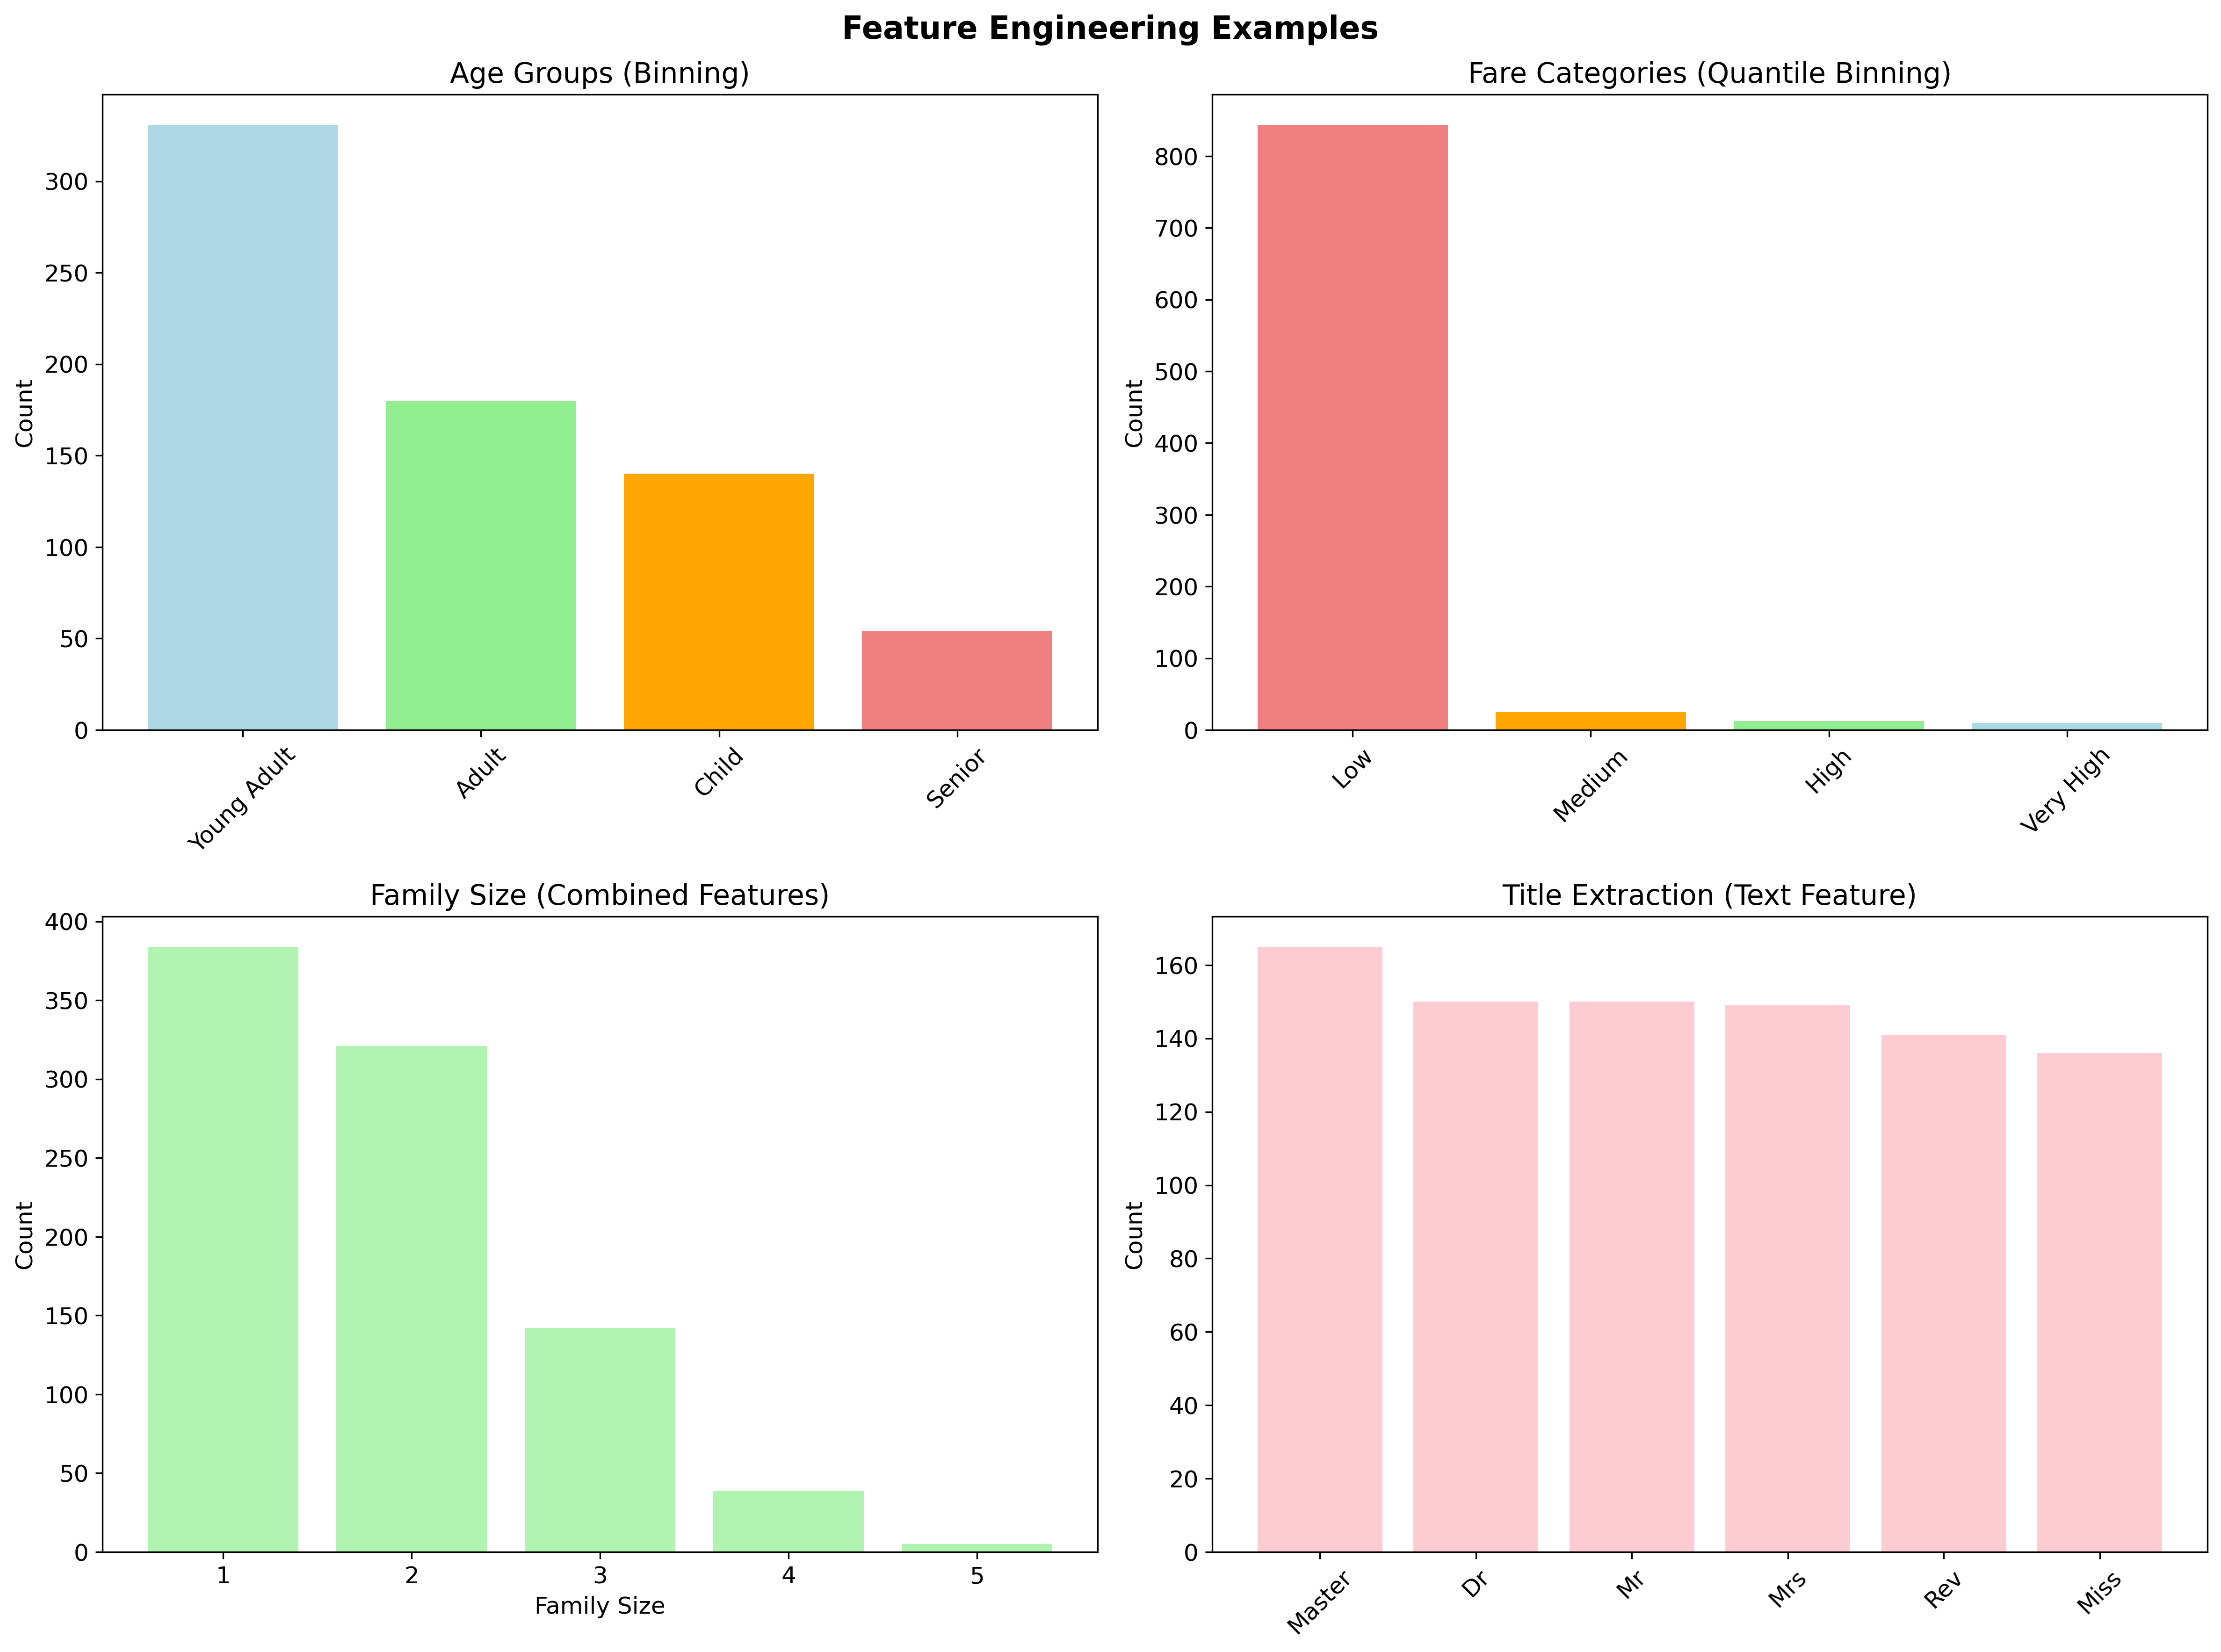
\includegraphics[width=0.9\textwidth]{../figures/07_feature_engineering.png}
\end{center}

\vspace{0.1cm}
\begin{alertblock}{Engineering Insights}
\textbf{Age binning:} Creates interpretable groups; \textbf{Family size:} Combines multiple features; \textbf{Title extraction:} Captures social status
\end{alertblock}
\end{frame}

\begin{frame}{Feature Creation Techniques}
\begin{columns}[t]
\begin{column}{0.48\textwidth}
\begin{block}{Binning \& Discretization}
\textbf{Equal-width binning:}
$$\text{bin width} = \frac{x_{\max} - x_{\min}}{k}$$

\textbf{Equal-frequency binning:}
Each bin contains $\frac{n}{k}$ observations

\textbf{Quantile-based binning:}
Based on percentiles (quartiles, deciles)

\textbf{Domain-specific binning:}
Using expert knowledge (e.g., age groups)
\end{block}

\vspace{0.1cm}
\begin{methodblock}{Optimal Binning}
Use information gain or chi-square test to determine optimal bin boundaries
\end{methodblock}
\end{column}

\begin{column}{0.48\textwidth}
\begin{block}{Feature Combinations}
\textbf{Arithmetic Operations:}
- Addition: $x_1 + x_2$ (total family size)
- Multiplication: $x_1 \times x_2$ (interaction terms)
- Division: $x_1 / x_2$ (ratios, rates)

\textbf{Boolean Operations:}
- Logical AND: $x_1 \land x_2$
- Logical OR: $x_1 \lor x_2$
- Conditional: if $x_1 > \text{threshold}$ then 1 else 0

\textbf{String Operations:}
- Length: $\text{len}(\text{string})$
- Contains: pattern matching
- Extract: regular expressions
\end{block}
\end{column}
\end{columns}

\begin{exampleblock}{Feature Engineering Guidelines}
\textbf{Domain Knowledge:} Most important factor; \textbf{Iterative Process:} Create, test, refine; \textbf{Validation:} Always validate on holdout set
\end{exampleblock}
\end{frame}

\begin{frame}{Mathematical Transformations}
\begin{columns}[t]
\begin{column}{0.48\textwidth}
\begin{block}{Power Transformations}
\textbf{Log Transformation:}
$$y = \log(x + c)$$
Reduces right skewness, stabilizes variance

\textbf{Square Root:}
$$y = \sqrt{x}$$
Moderate variance stabilization

\textbf{Box-Cox Transformation:}
$$y = \begin{cases}
\frac{x^\lambda - 1}{\lambda} & \text{if } \lambda \neq 0 \\
\ln(x) & \text{if } \lambda = 0
\end{cases}$$

Optimal $\lambda$ found via maximum likelihood
\end{block}
\end{column}

\begin{column}{0.48\textwidth}
\begin{block}{Trigonometric Features}
For cyclical data (time, angles):

\textbf{Sine/Cosine encoding:}
$$\sin\left(\frac{2\pi \times \text{value}}{\text{max\_value}}\right)$$
$$\cos\left(\frac{2\pi \times \text{value}}{\text{max\_value}}\right)$$

\textbf{Example for hour of day:}
$$\text{hour\_sin} = \sin\left(\frac{2\pi \times \text{hour}}{24}\right)$$
$$\text{hour\_cos} = \cos\left(\frac{2\pi \times \text{hour}}{24}\right)$$
\end{block}

\vspace{0.1cm}
\begin{tipblock}{When to Transform}
Transform when: skewed data, non-linear relationships, or specific model requirements
\end{tipblock}
\end{column}
\end{columns}
\end{frame}

% ========================================
% Section: Feature Selection
% ========================================

\section{Feature Selection}

\begin{frame}{Feature Selection Methods}
\begin{center}
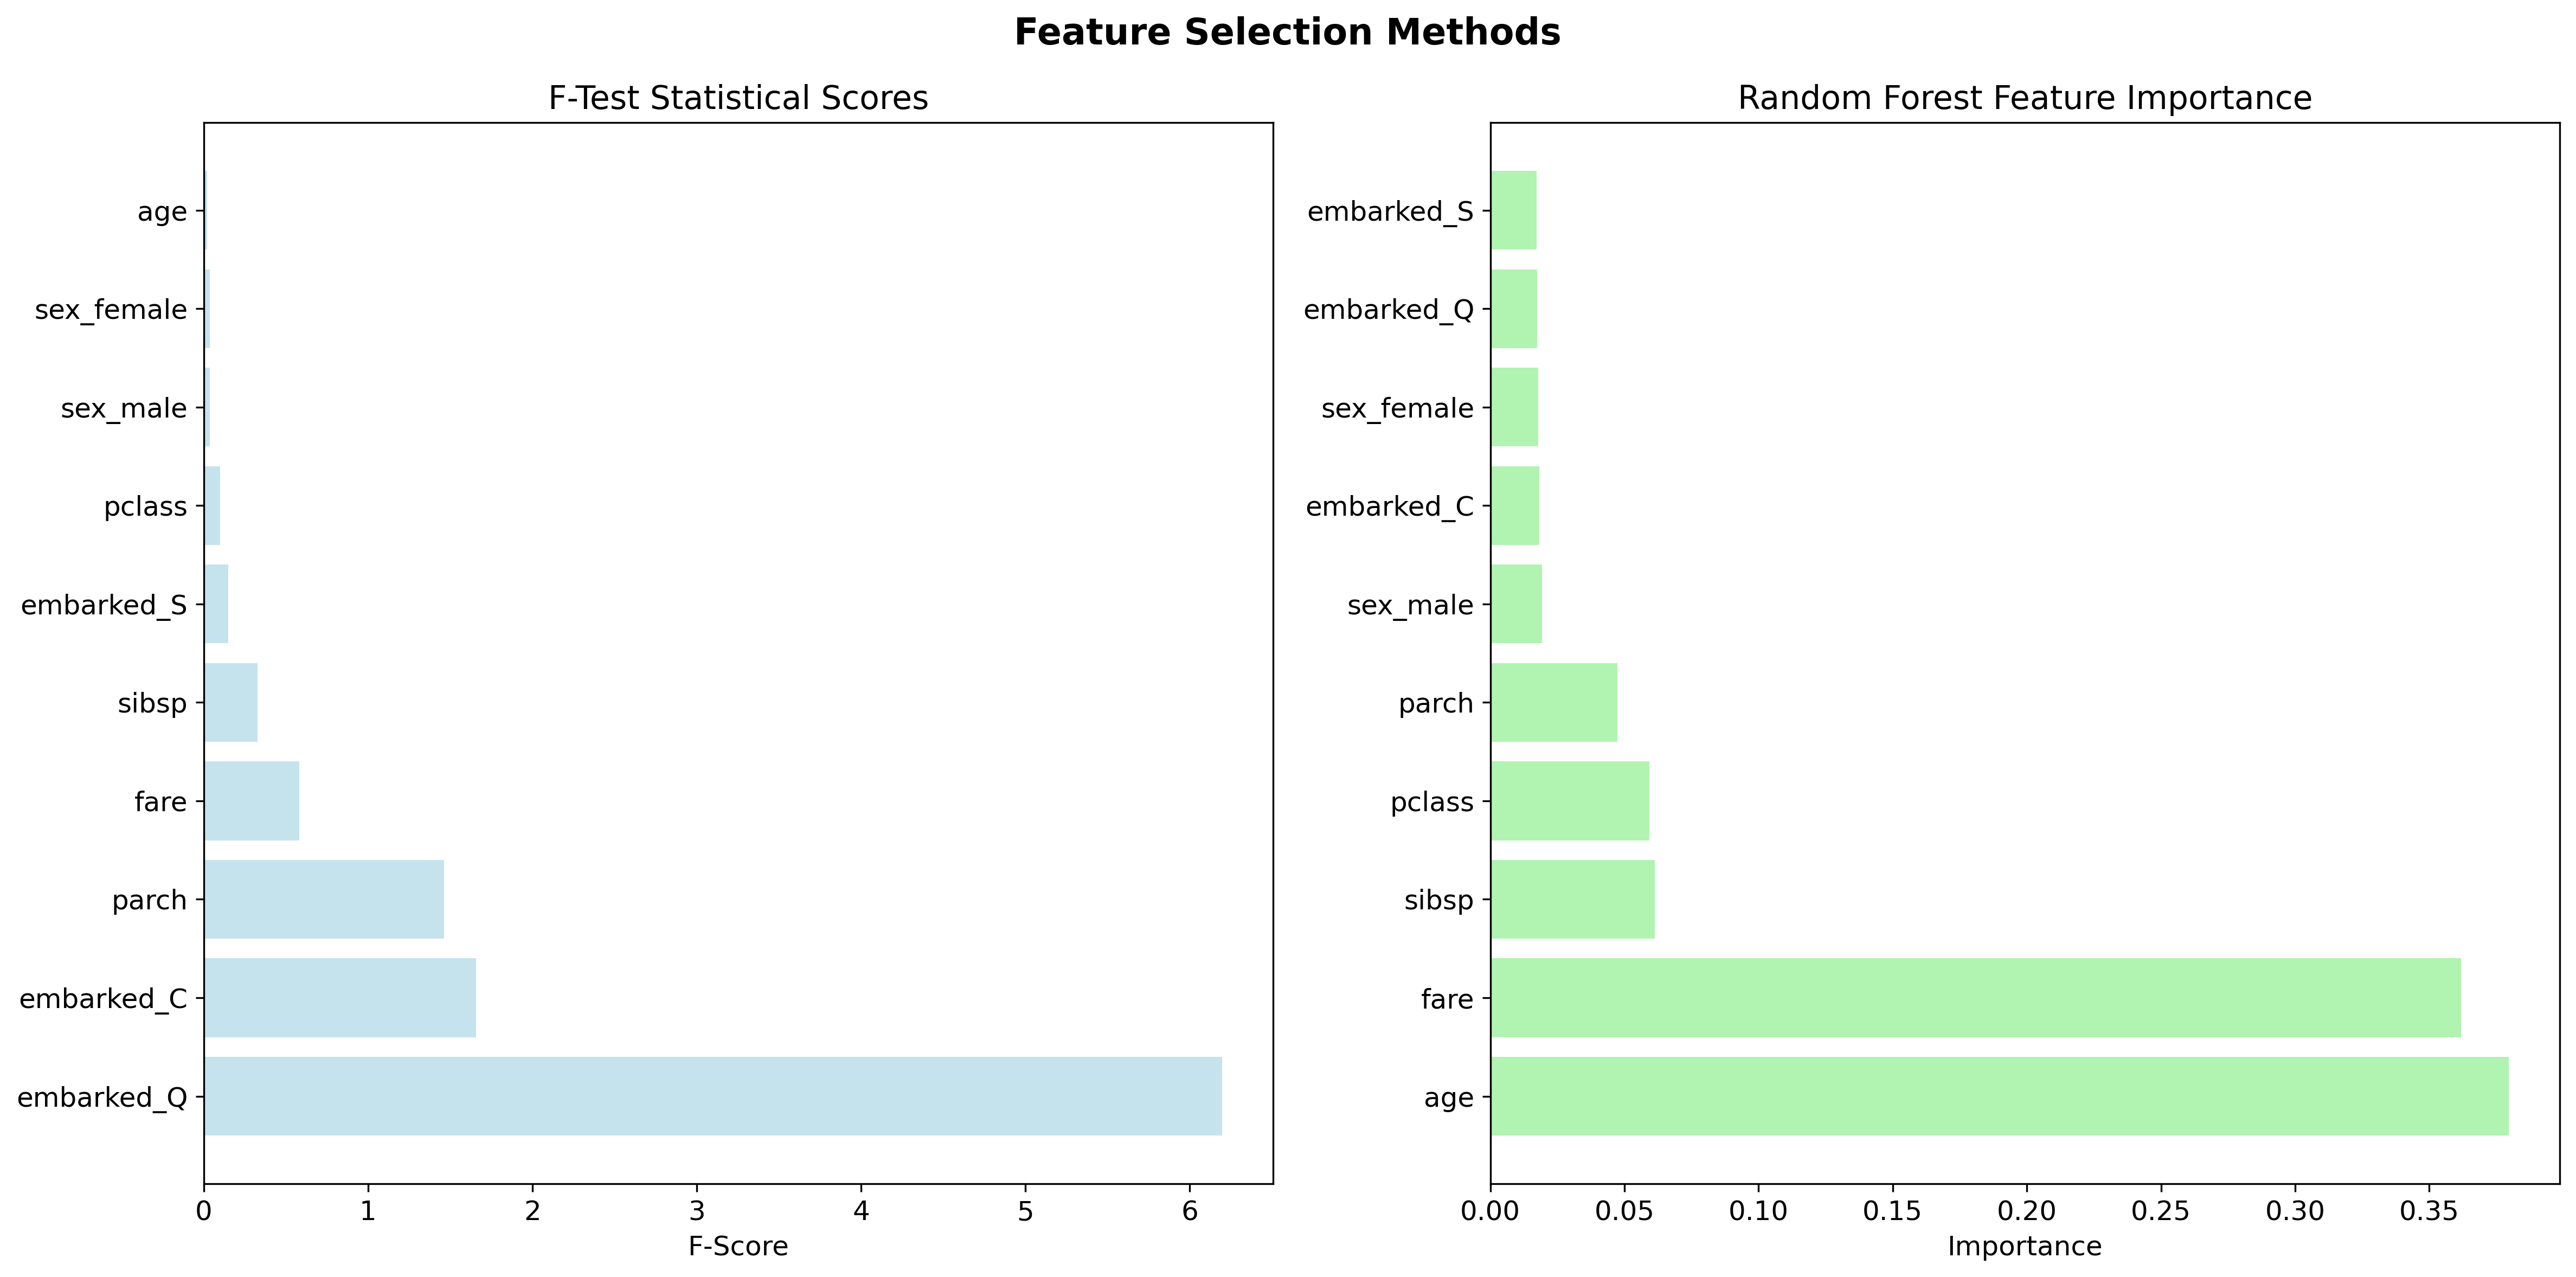
\includegraphics[width=0.9\textwidth]{../figures/09_feature_selection.png}
\end{center}

\vspace{0.1cm}
\begin{alertblock}{Selection Results}
\textbf{Statistical:} Gender and fare most important; \textbf{Tree-based:} Consistent with domain knowledge about survival factors
\end{alertblock}
\end{frame}

\begin{frame}{Statistical Feature Selection}
\begin{columns}[t]
\begin{column}{0.48\textwidth}
\begin{block}{Filter Methods}
\textbf{Correlation-based:}
Select features with high correlation to target, low correlation to each other

\textbf{F-test (ANOVA):}
$$F = \frac{\text{MSB}}{\text{MSW}} = \frac{\sum_{i=1}^k n_i(\bar{x}_i - \bar{x})^2/(k-1)}{\sum_{i=1}^k \sum_{j=1}^{n_i}(x_{ij} - \bar{x}_i)^2/(n-k)}$$

\textbf{Chi-square test:}
$$\chi^2 = \sum_{i,j} \frac{(O_{ij} - E_{ij})^2}{E_{ij}}$$

\textbf{Mutual Information:}
$$I(X;Y) = \sum_{x,y} p(x,y) \log \frac{p(x,y)}{p(x)p(y)}$$
\end{block}
\end{column}

\begin{column}{0.48\textwidth}
\begin{block}{Wrapper Methods}
\textbf{Forward Selection:}
Start with empty set, add best features iteratively

\textbf{Backward Elimination:}
Start with all features, remove worst iteratively

\textbf{Recursive Feature Elimination:}
$$\text{rank}_i = f(\text{coef}_i, \text{importance}_i)$$

\textbf{Genetic Algorithm:}
Evolutionary approach to feature subset selection
\end{block}

\vspace{0.1cm}
\begin{methodblock}{Embedded Methods}
\textbf{L1 Regularization (Lasso):}
$$\min_\beta \frac{1}{2n}||y - X\beta||^2_2 + \lambda||\beta||_1$$
\end{methodblock}
\end{column}
\end{columns}
\end{frame}

\begin{frame}{Tree-based Feature Importance}
\begin{columns}[t]
\begin{column}{0.48\textwidth}
\begin{block}{Random Forest Importance}
\textbf{Mean Decrease Impurity:}
$$\text{Importance}(x_j) = \frac{1}{T}\sum_{t=1}^T \sum_{v \in \text{splits}} p(v) \times \Delta I(v)$$

where:
- $T$ = number of trees
- $p(v)$ = proportion of samples reaching node $v$
- $\Delta I(v)$ = impurity decrease at node $v$

\textbf{Mean Decrease Accuracy:}
Permutation-based importance measuring prediction accuracy drop when feature is shuffled
\end{block}
\end{column}

\begin{column}{0.48\textwidth}
\begin{block}{Gradient Boosting Importance}
\textbf{Gain-based Importance:}
$$\text{Importance}(x_j) = \sum_{t=1}^T \sum_{v \in \text{splits}_j} \text{gain}(v)$$

\textbf{SHAP Values:}
Shapley Additive exPlanations provide unified measure:
$$\phi_j = \sum_{S \subseteq N \setminus \{j\}} \frac{|S|!(|N|-|S|-1)!}{|N|!}[f(S \cup \{j\}) - f(S)]$$
\end{block}

\vspace{0.1cm}
\begin{alertblock}{Caution}
Tree-based importance can be biased toward high-cardinality categorical features
\end{alertblock}
\end{column}
\end{columns}
\end{frame}

% ========================================
% Section: Data Normalization
% ========================================

\section{Data Normalization}

\begin{frame}{Normalization Comparison}
\begin{center}
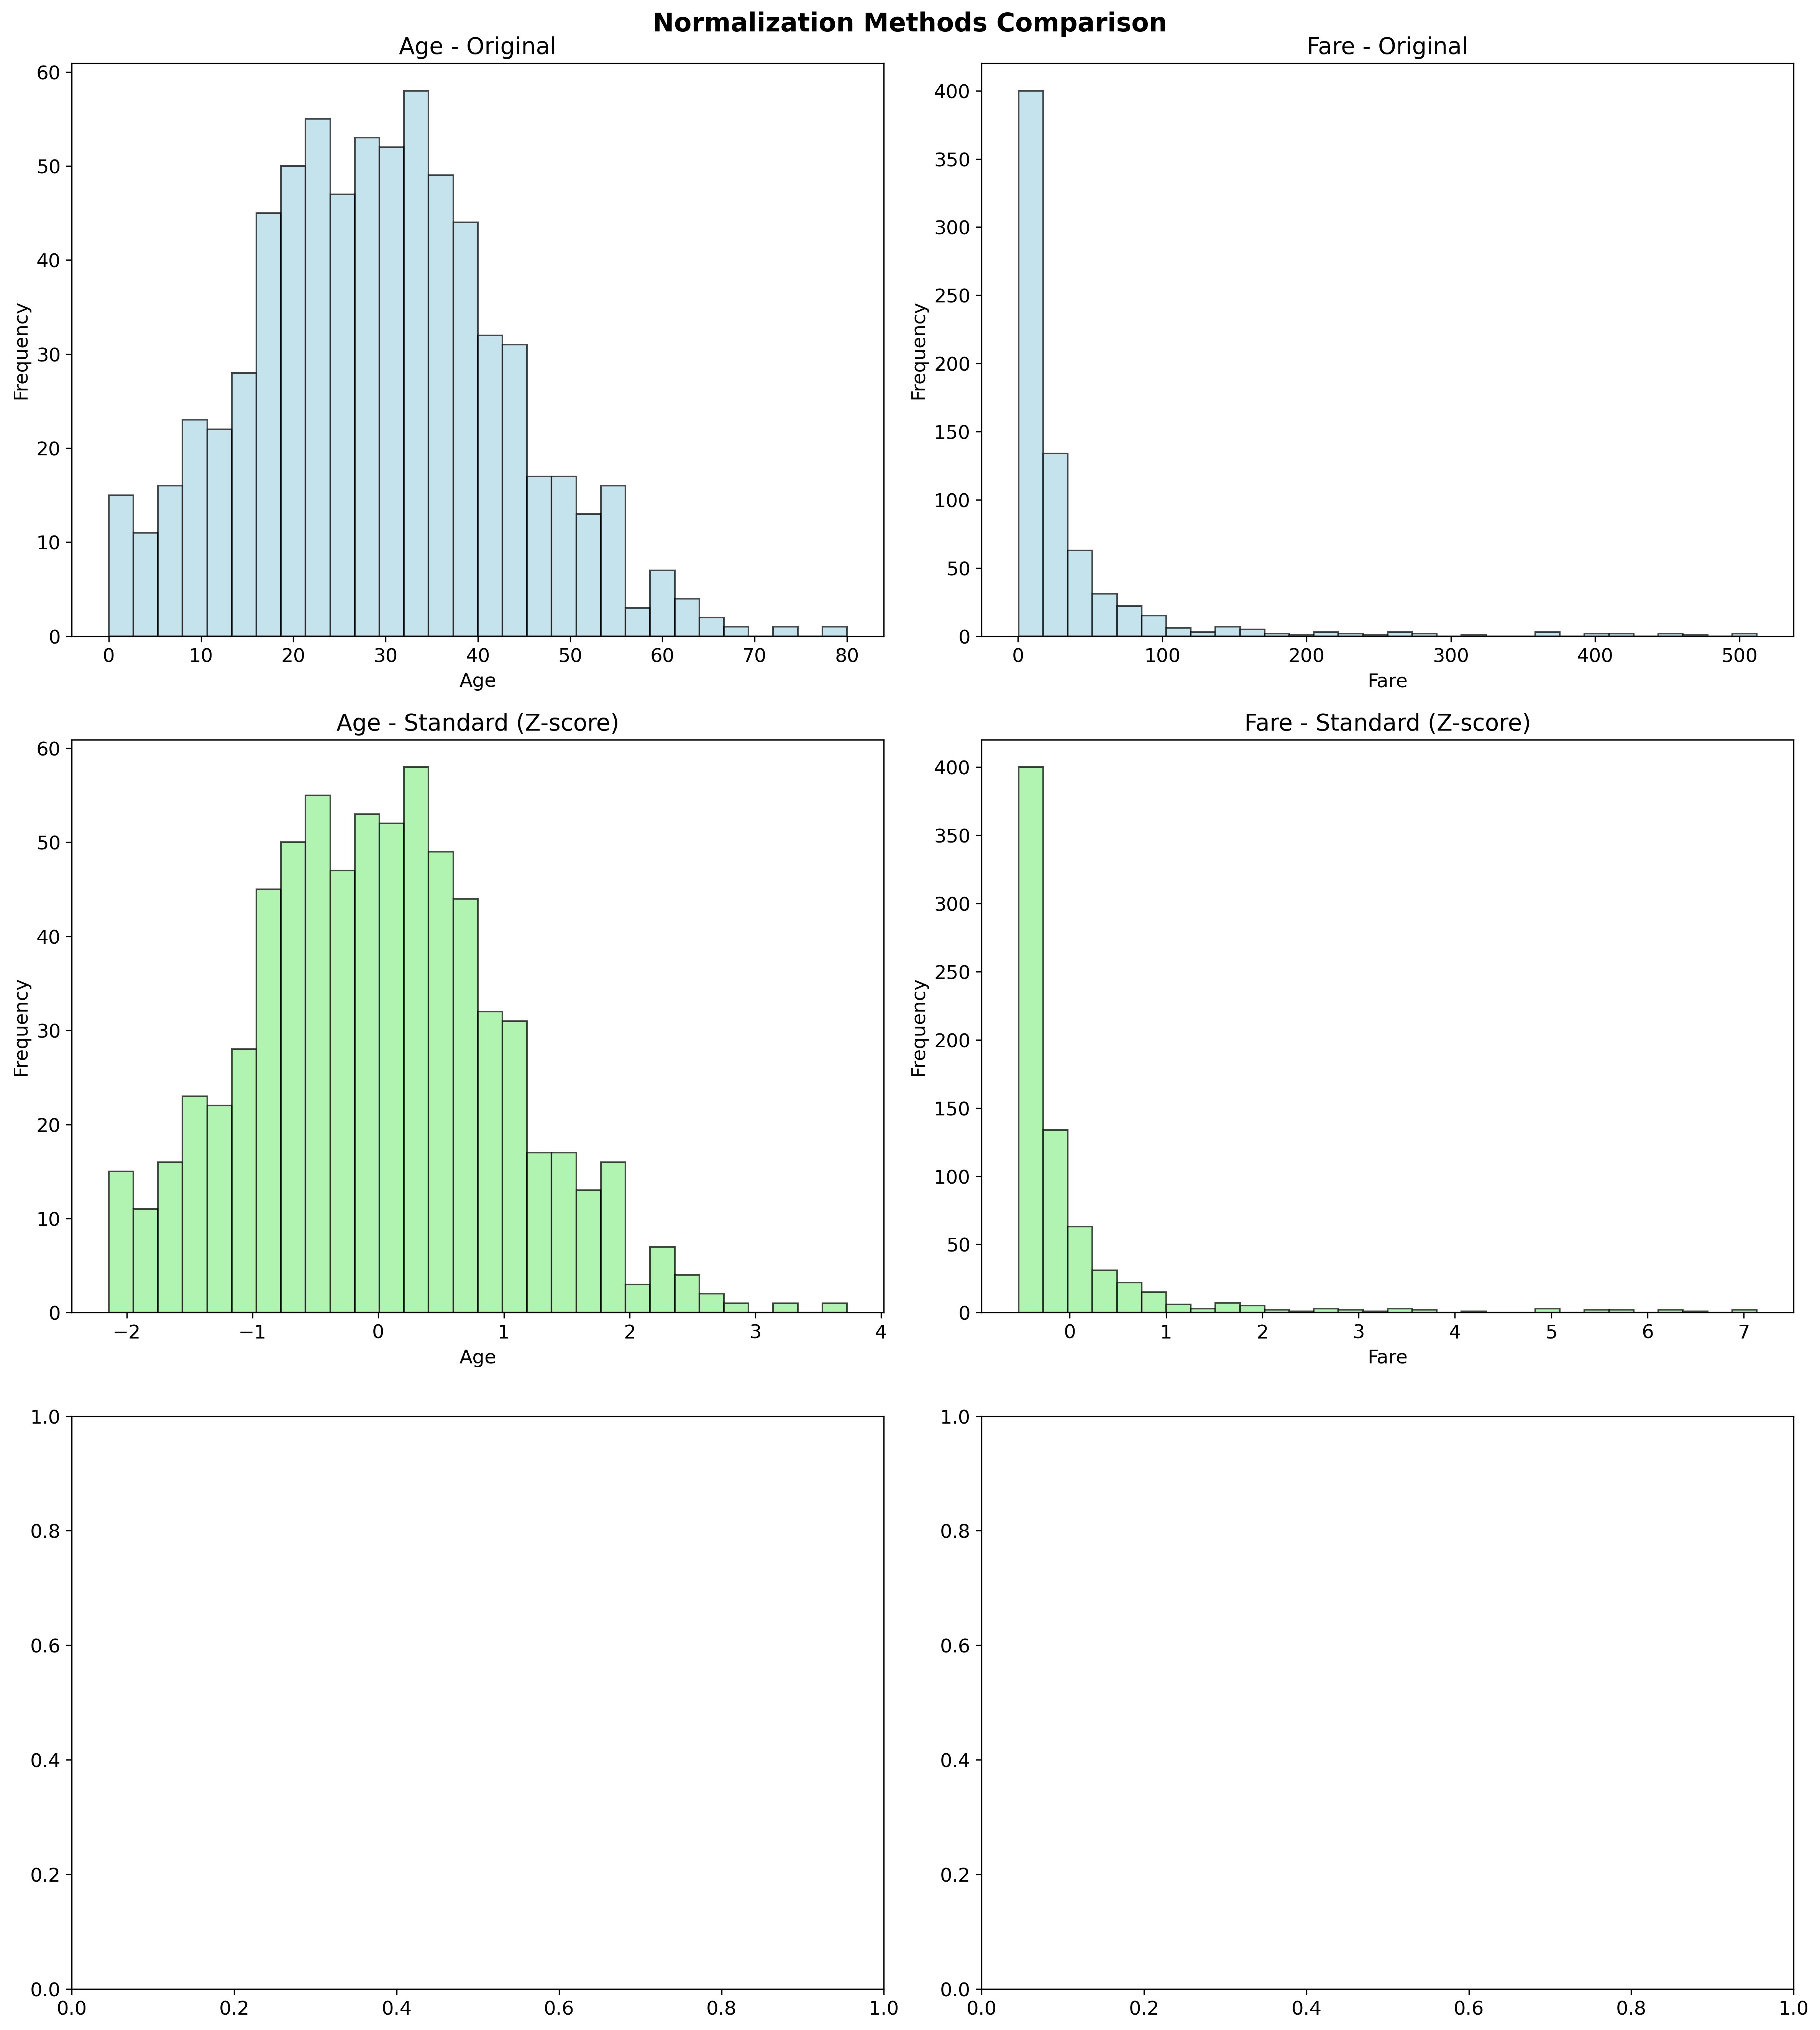
\includegraphics[width=0.9\textwidth]{../figures/08_normalization_comparison.png}
\end{center}

\vspace{0.1cm}
\begin{alertblock}{Normalization Effects}
\textbf{StandardScaler:} Zero mean, unit variance; \textbf{MinMaxScaler:} [0,1] range; \textbf{RobustScaler:} Median-based, outlier resistant
\end{alertblock}
\end{frame}

\begin{frame}{Scaling Methods Mathematical Formulations}
\begin{columns}[t]
\begin{column}{0.48\textwidth}
\begin{block}{Standard Scaling (Z-score)}
$$x_{\text{scaled}} = \frac{x - \mu}{\sigma}$$

where $\mu = \frac{1}{n}\sum_{i=1}^n x_i$ and $\sigma = \sqrt{\frac{1}{n-1}\sum_{i=1}^n (x_i - \mu)^2}$

\textbf{Properties:}
- Mean = 0, Std = 1
- Preserves distribution shape
- Sensitive to outliers
\end{block}

\vspace{0.1cm}
\begin{block}{Min-Max Scaling}
$$x_{\text{scaled}} = \frac{x - x_{\min}}{x_{\max} - x_{\min}}$$

\textbf{Properties:}
- Range: [0, 1]
- Preserves relationships
- Very sensitive to outliers
\end{block}
\end{column}

\begin{column}{0.48\textwidth}
\begin{block}{Robust Scaling}
$$x_{\text{scaled}} = \frac{x - \text{Median}(x)}{\text{IQR}(x)}$$

where $\text{IQR} = Q_3 - Q_1$

\textbf{Properties:}
- Median-centered
- Uses interquartile range
- Robust to outliers
\end{block}

\vspace{0.1cm}
\begin{block}{Unit Vector Scaling}
$$x_{\text{scaled}} = \frac{x}{||x||_2}$$

where $||x||_2 = \sqrt{\sum_{i=1}^n x_i^2}$

\textbf{Use case:} When magnitude matters more than individual values
\end{block}
\end{column}
\end{columns}

\begin{tipblock}{Selection Guide}
\textbf{Normal data + no outliers:} StandardScaler; \textbf{Bounded range needed:} MinMaxScaler; \textbf{Outliers present:} RobustScaler
\end{tipblock}
\end{frame}

\begin{frame}{When \& Why to Normalize}
\begin{columns}[t]
\begin{column}{0.48\textwidth}
\begin{block}{Algorithms Requiring Normalization}
\textbf{Distance-based:}
- k-NN, k-means clustering
- SVM with RBF kernel
- Neural networks

\textbf{Gradient-based:}
- Logistic regression
- Linear regression with regularization
- Deep learning

\textbf{Mathematical justification:}
Features with larger scales dominate distance calculations:
$$d = \sqrt{\sum_{i=1}^p (x_i - y_i)^2}$$
\end{block}
\end{column}

\begin{column}{0.48\textwidth}
\begin{block}{Algorithms Not Requiring Normalization}
\textbf{Tree-based methods:}
- Decision trees
- Random Forest
- Gradient boosting

\textbf{Reason:} Trees use split points, not absolute values

\textbf{Rule-based:}
- Naive Bayes
- Association rules

\textbf{Statistical:} Feature scales don't affect splitting decisions or probability calculations
\end{block}
\end{column}
\end{columns}

\vspace{0.1cm}
\begin{alertblock}{Critical Rule}
\textbf{Always fit scaler on training data only!} Apply same transformation to validation/test sets to avoid data leakage.
\end{alertblock}
\end{frame}

% ========================================
% Section: Advanced Topics
% ========================================

\section{Advanced EDA Topics}

\begin{frame}{Target Variable Analysis}
\begin{center}
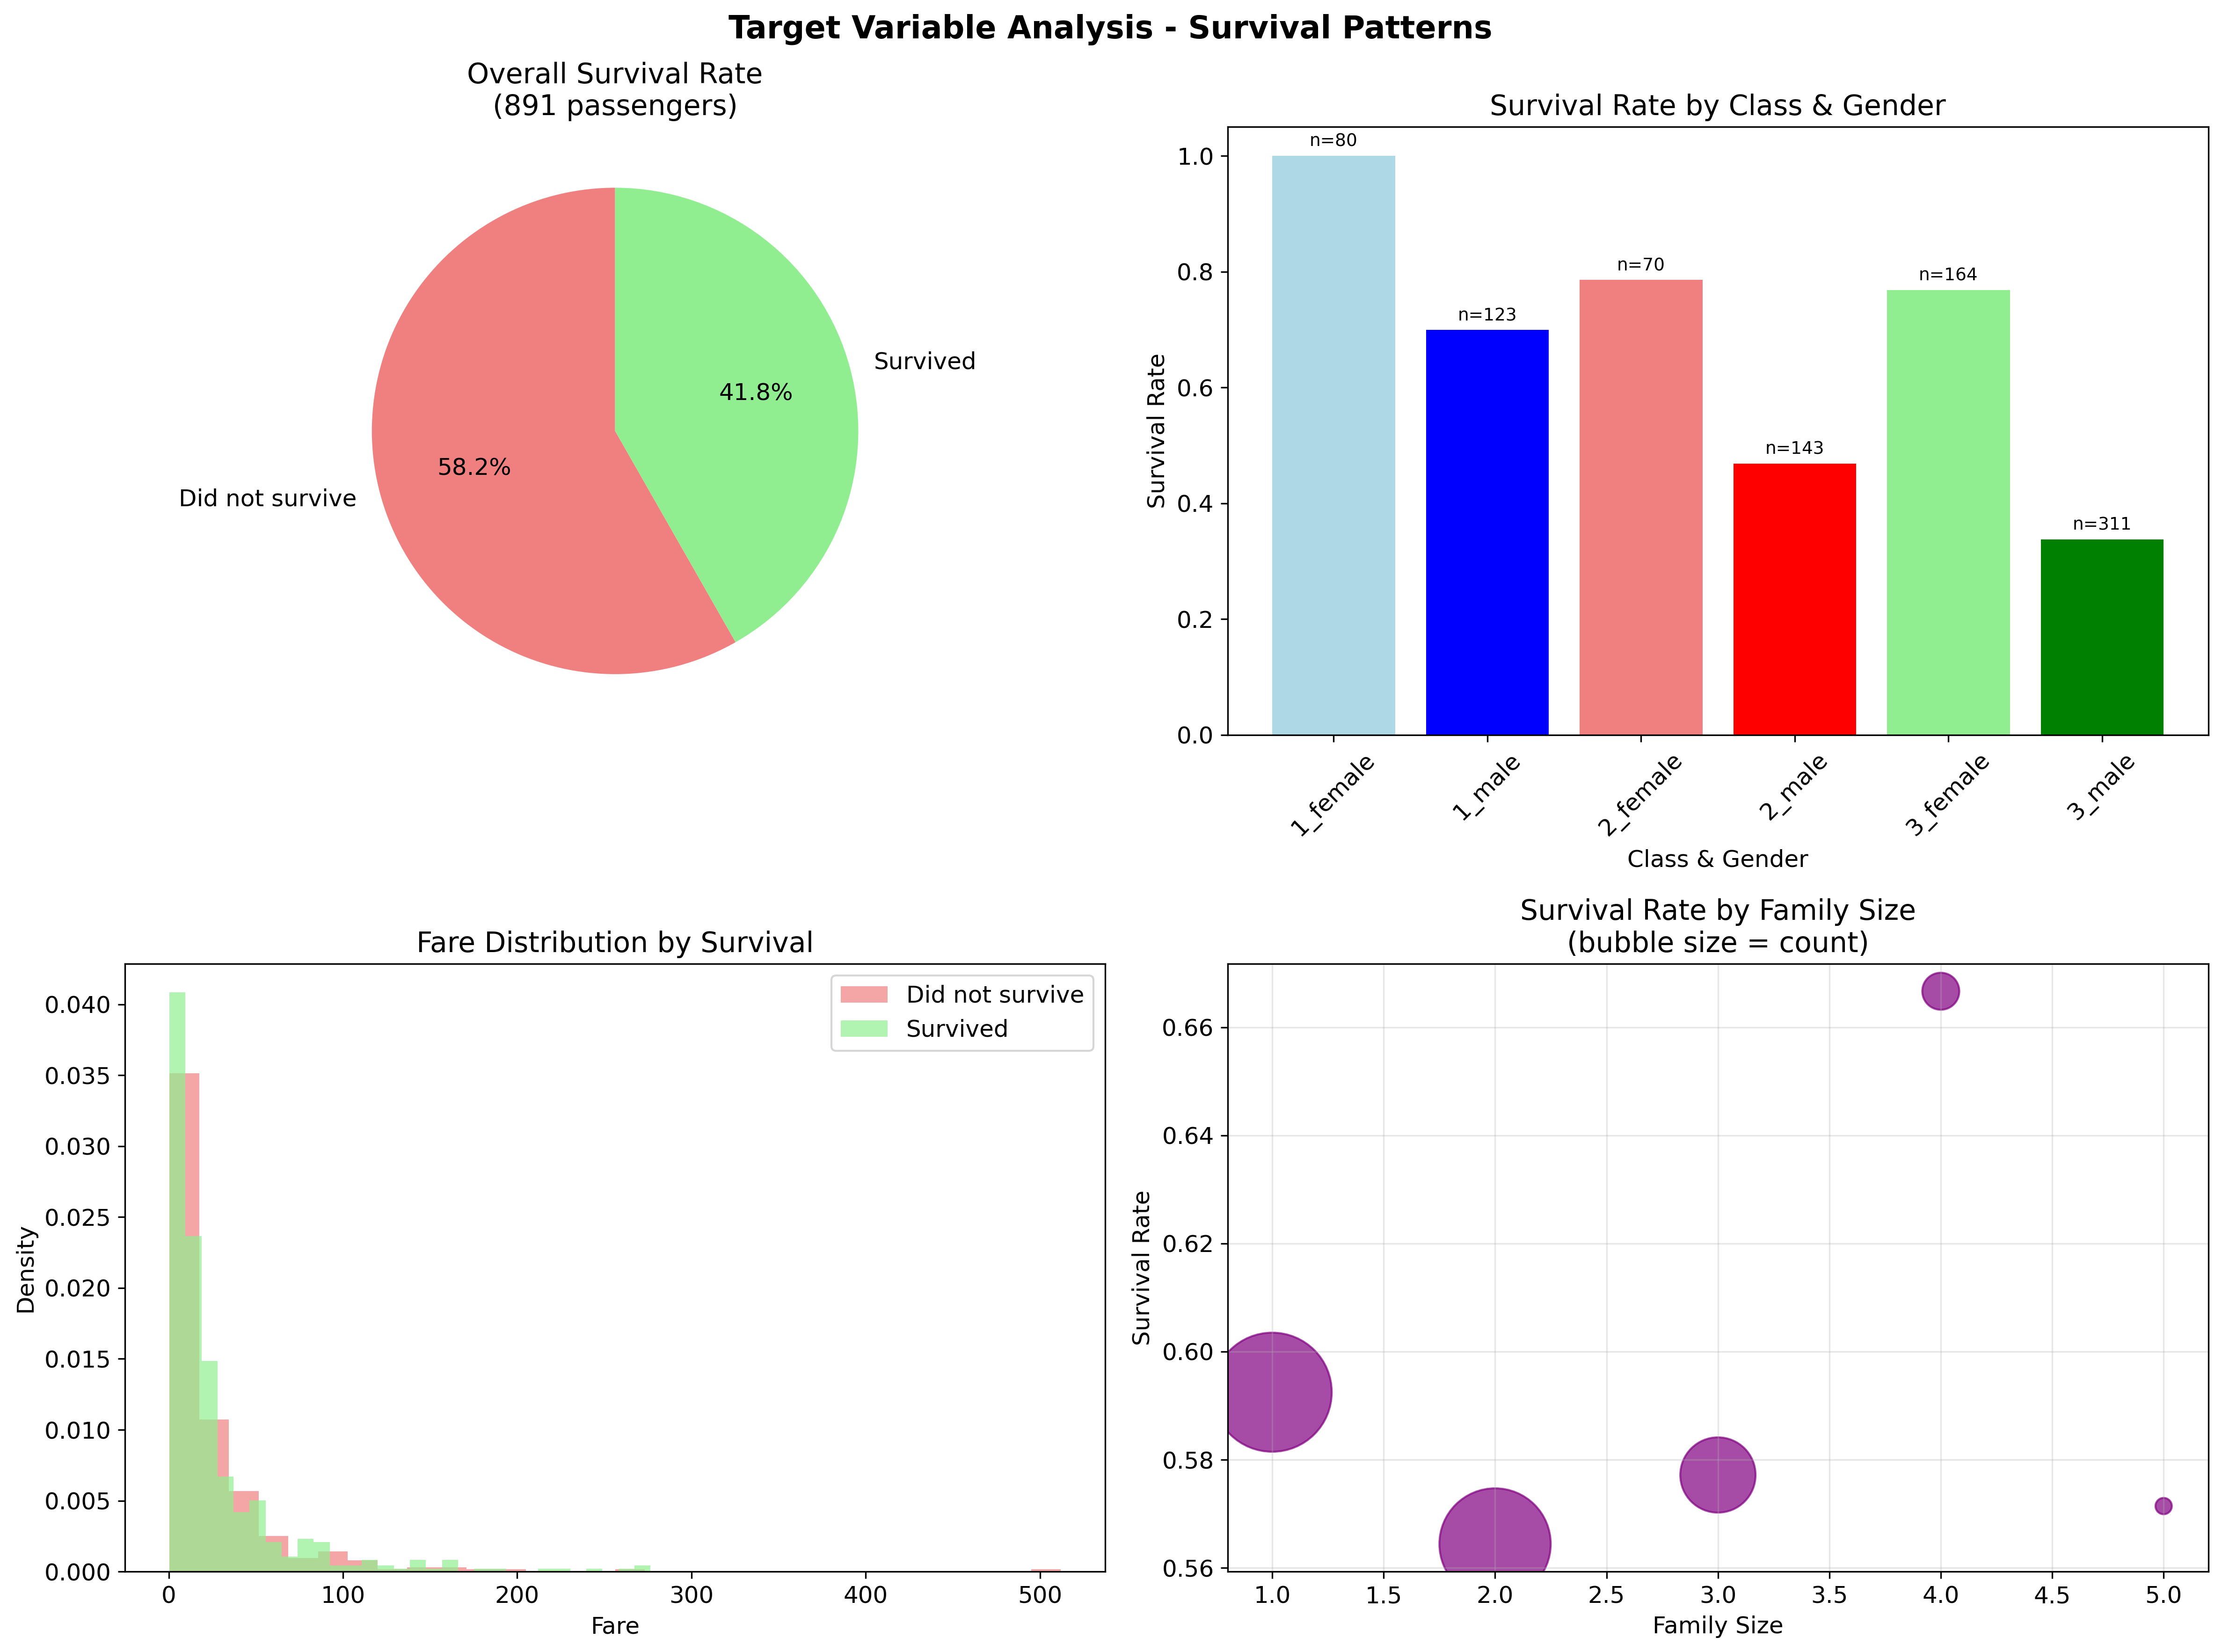
\includegraphics[width=0.9\textwidth]{../figures/11_target_analysis.png}
\end{center}

\vspace{0.1cm}
\begin{alertblock}{Target Insights}
\textbf{Class imbalance:} 62\% non-survival; \textbf{Gender-class interaction:} First-class women had 97\% survival rate
\end{alertblock}
\end{frame}

\begin{frame}{Business Insights from EDA}
\begin{center}
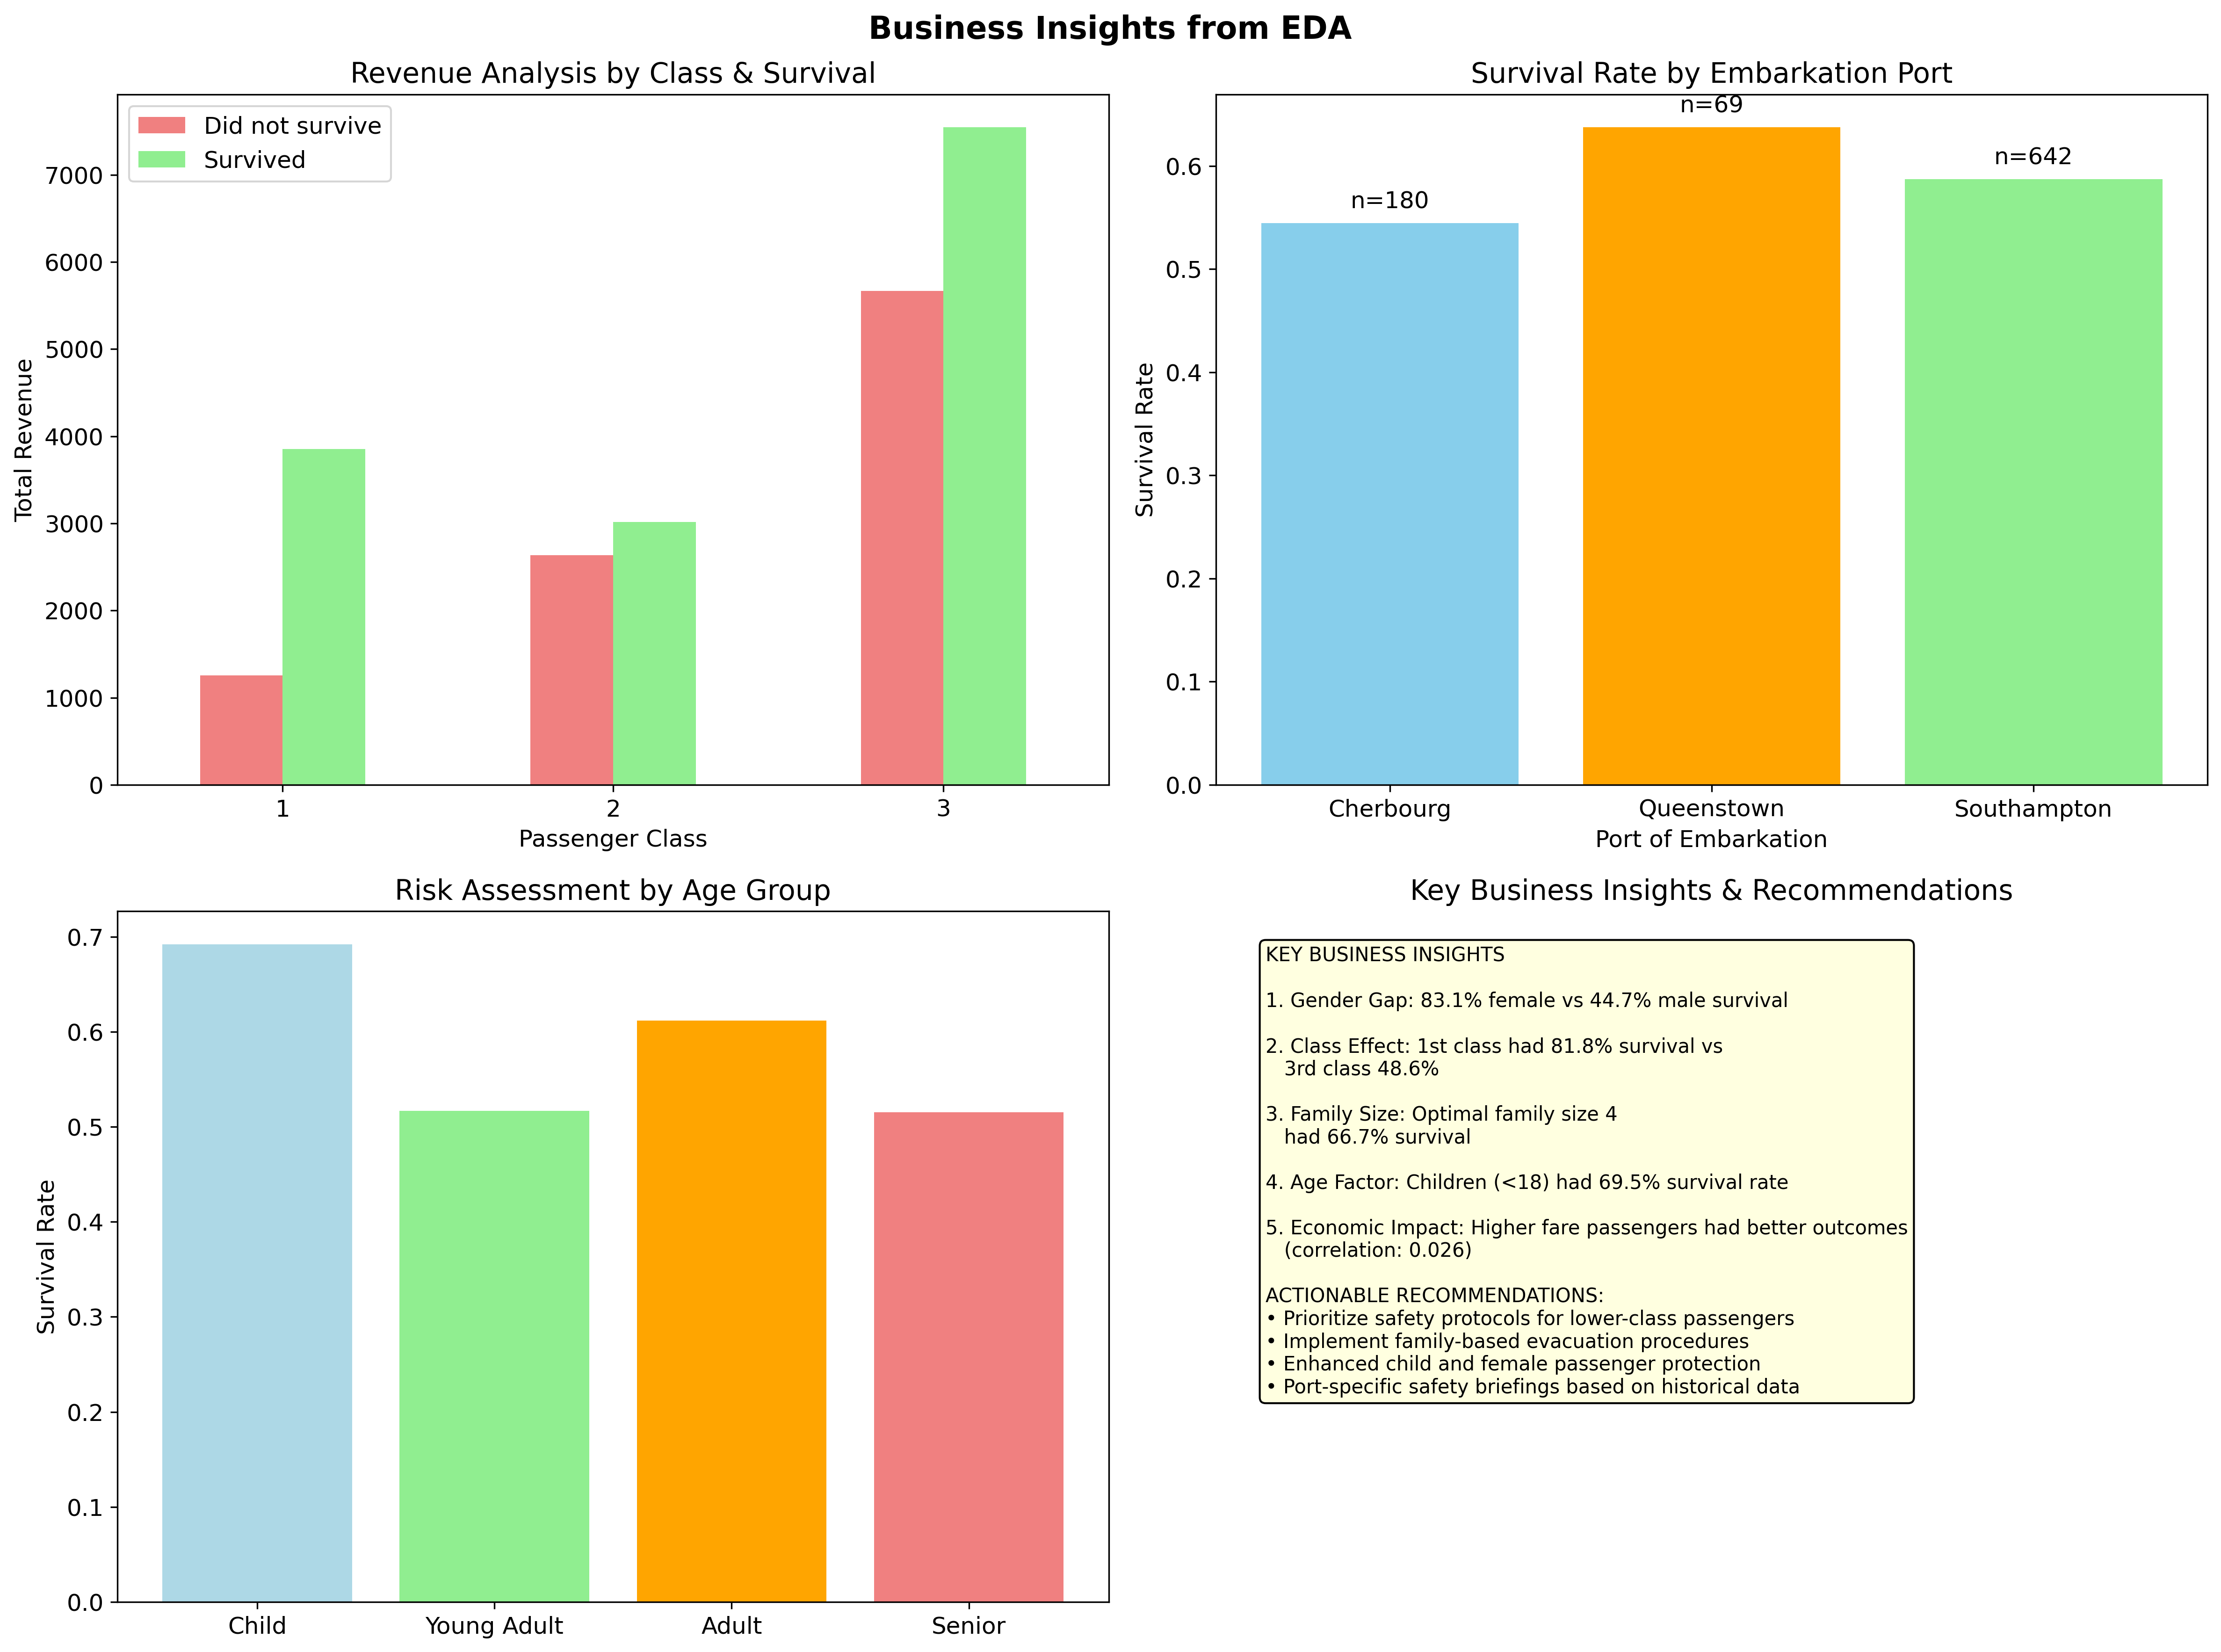
\includegraphics[width=0.9\textwidth]{../figures/12_business_insights.png}
\end{center}

\vspace{0.1cm}
\begin{alertblock}{Actionable Insights}
\textbf{Revenue impact:} Higher-paying passengers had better survival rates; \textbf{Port differences:} Embarkation port correlates with survival
\end{alertblock}
\end{frame}

\begin{frame}{Advanced Visualization Techniques}
\begin{columns}[t]
\begin{column}{0.48\textwidth}
\begin{block}{Dimensionality Reduction}
\textbf{Principal Component Analysis:}
$$\mathbf{Y} = \mathbf{XW}$$
where $\mathbf{W}$ contains eigenvectors of covariance matrix

\textbf{t-SNE:}
$$p_{j|i} = \frac{\exp(-||\mathbf{x}_i - \mathbf{x}_j||^2/2\sigma_i^2)}{\sum_{k \neq i} \exp(-||\mathbf{x}_i - \mathbf{x}_k||^2/2\sigma_i^2)}$$

\textbf{UMAP:} Uniform Manifold Approximation
- Preserves local and global structure
- Faster than t-SNE
- Better for clustering visualization
\end{block}
\end{column}

\begin{column}{0.48\textwidth}
\begin{block}{Interactive Visualizations}
\textbf{Plotly Benefits:}
- Zoom, pan, hover information
- 3D scatter plots
- Animated visualizations
- Dashboard creation

\textbf{Parallel Coordinates:}
Visualize high-dimensional data relationships

\textbf{Sankey Diagrams:}
Show flow between categorical variables

\textbf{Radar Charts:}
Compare multiple features simultaneously
\end{block}
\end{column}
\end{columns}

\vspace{0.1cm}
\begin{tipblock}{Best Practice}
\textbf{Progressive Disclosure:} Start with simple plots, add complexity as needed for deeper insights
\end{tipblock}
\end{frame}

\begin{frame}{Time Series EDA Considerations}
\begin{columns}[t]
\begin{column}{0.48\textwidth}
\begin{block}{Time Series Components}
\textbf{Decomposition:}
$$y(t) = \text{Trend}(t) + \text{Seasonal}(t) + \text{Noise}(t)$$

\textbf{Stationarity Testing:}
Augmented Dickey-Fuller test:
$$\Delta y_t = \alpha + \beta t + \gamma y_{t-1} + \delta_1 \Delta y_{t-1} + \cdots + \epsilon_t$$

\textbf{Autocorrelation:}
$$\rho_k = \frac{\text{Cov}(y_t, y_{t-k})}{\text{Var}(y_t)}$$
\end{block}
\end{column}

\begin{column}{0.48\textwidth}
\begin{block}{Seasonal Analysis}
\textbf{Seasonal Decomposition:}
- STL (Seasonal and Trend decomposition using Loess)
- X-12-ARIMA
- Classical decomposition

\textbf{Periodogram:}
$$I(\omega) = \frac{1}{n}\left|\sum_{t=1}^n y_t e^{-i\omega t}\right|^2$$

\textbf{Box-Cox for stabilization:}
Handle changing variance over time
\end{block}
\end{column}
\end{columns}

\vspace{0.1cm}
\begin{alertblock}{Time Series EDA Goals}
Identify trends, seasonality, outliers, structural breaks, and appropriate transformation needs
\end{alertblock}
\end{frame}

% ========================================
% Section: EDA to ML Pipeline
% ========================================

\section{EDA to ML Pipeline Integration}

\begin{frame}{EDA to ML Pipeline Integration}
\begin{center}
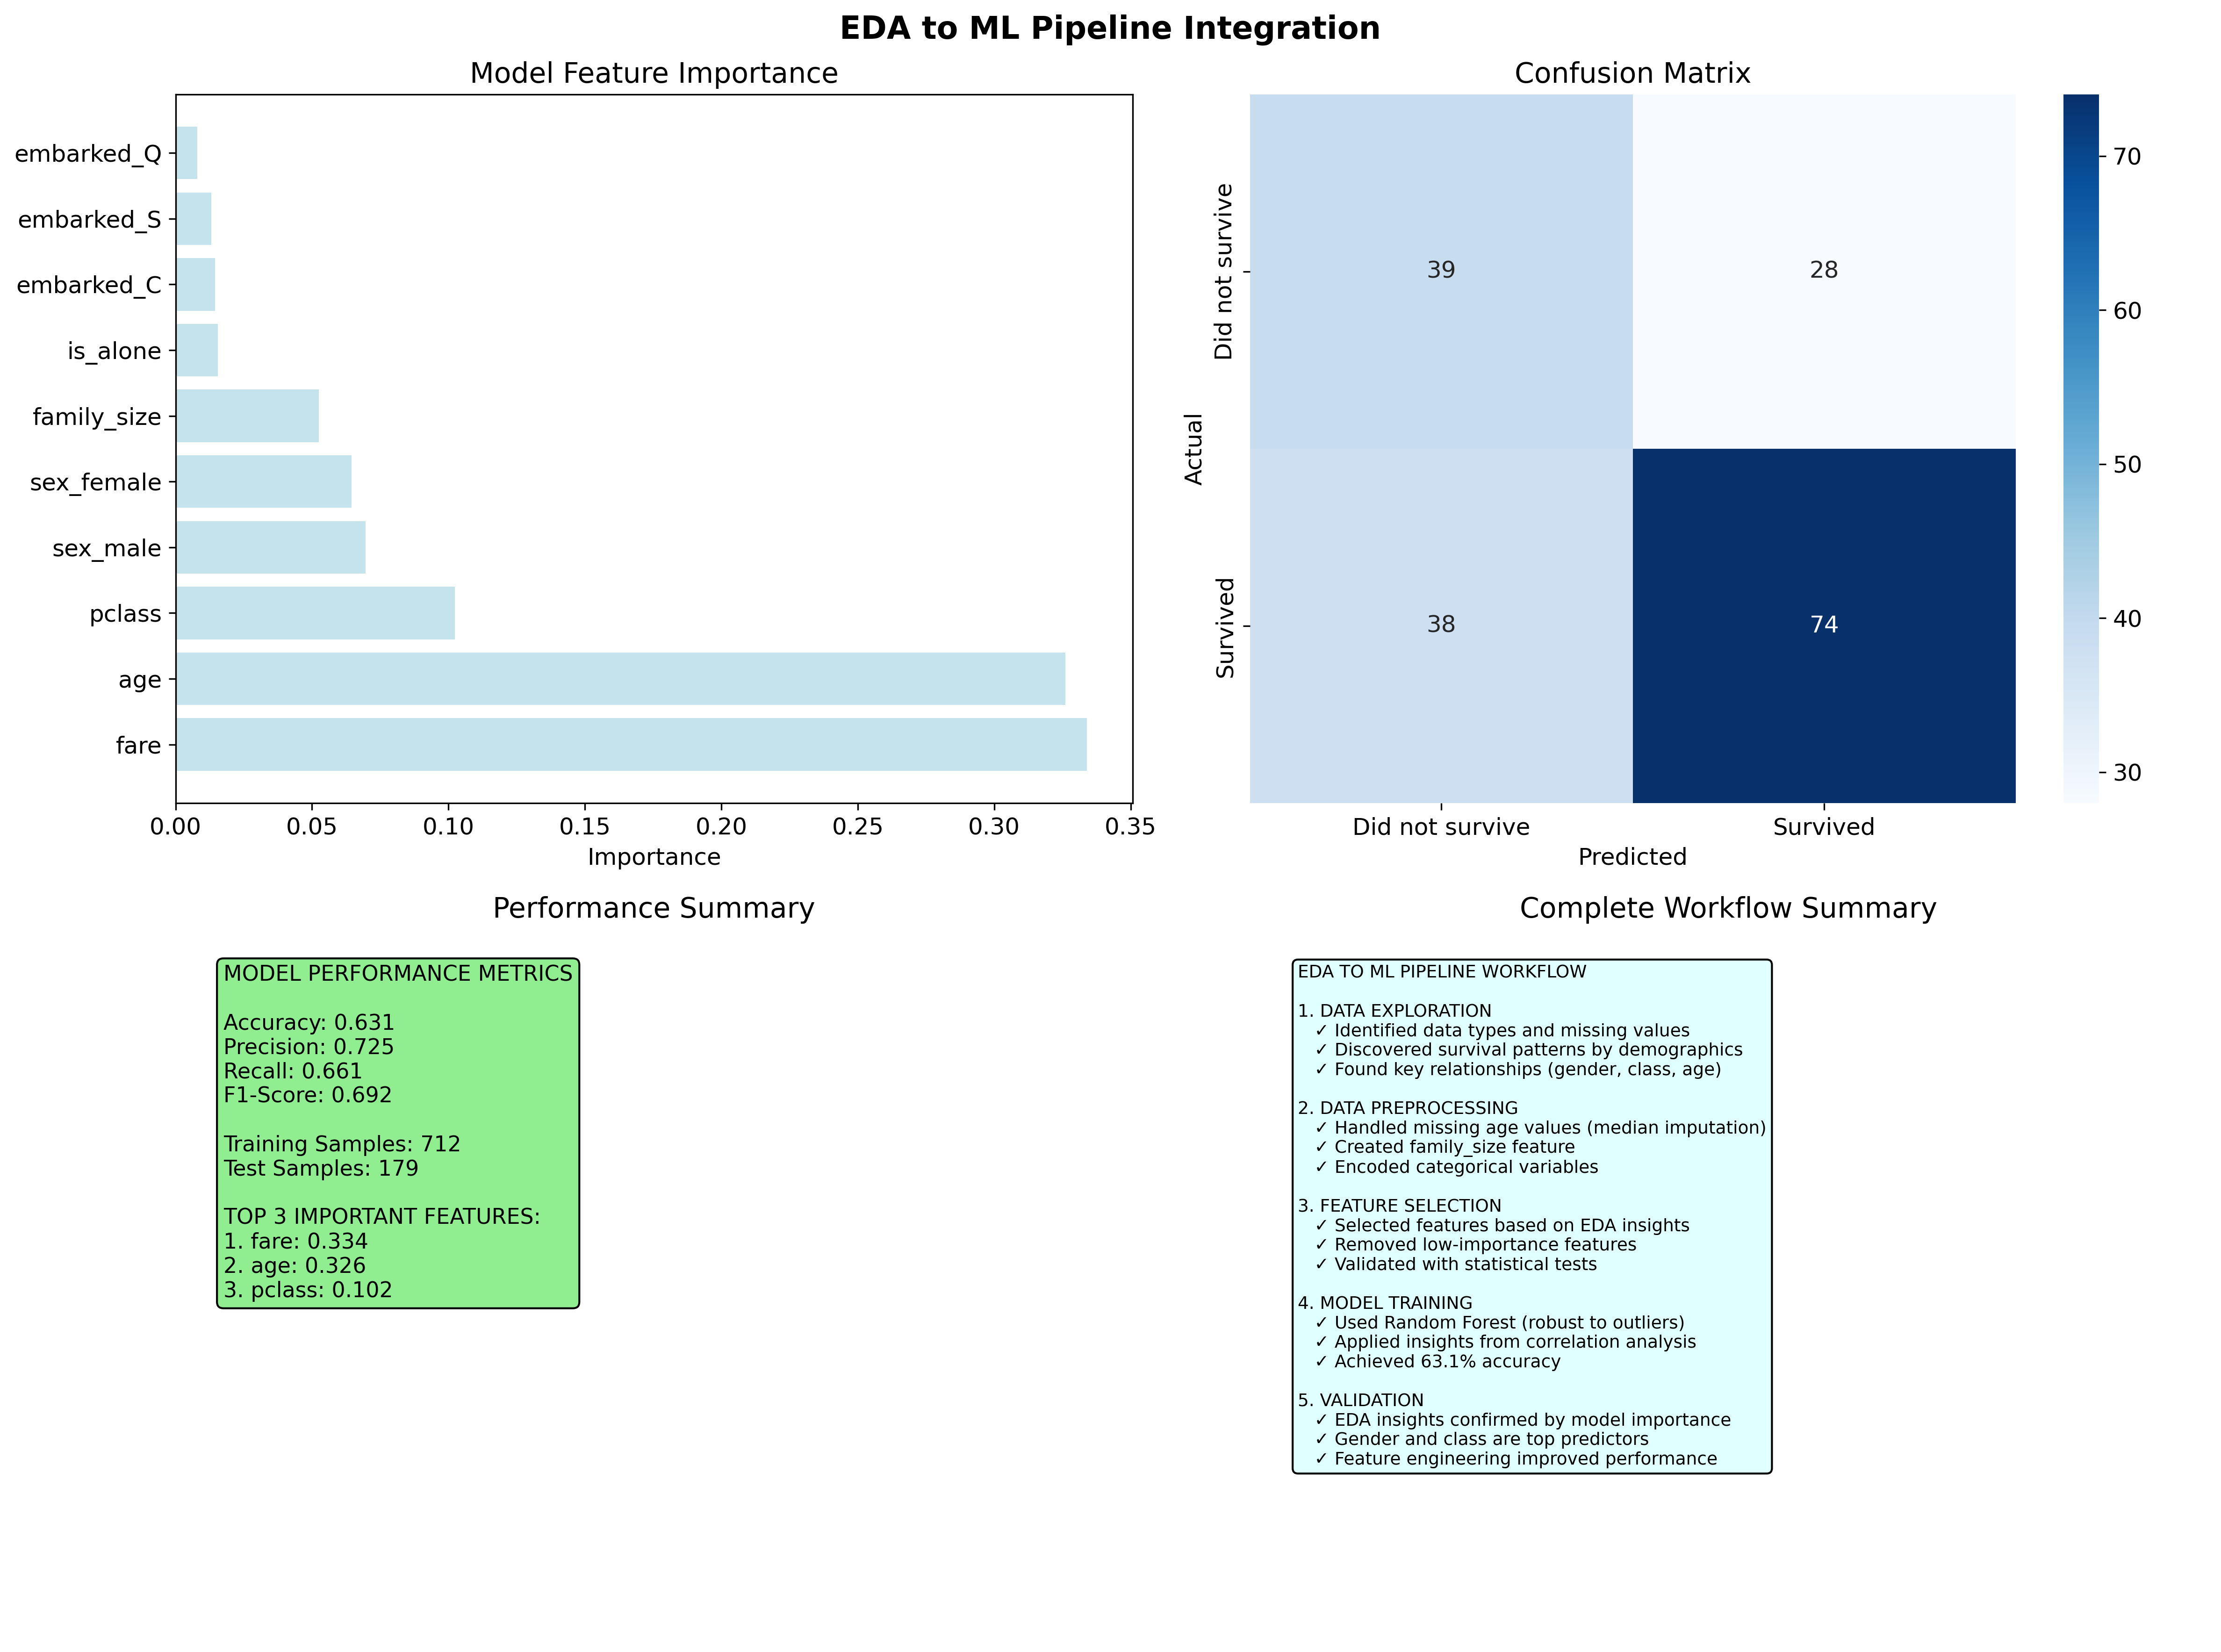
\includegraphics[width=0.9\textwidth]{../figures/13_ml_pipeline_demo.png}
\end{center}

\vspace{0.1cm}
\begin{alertblock}{Pipeline Success}
\textbf{EDA insights validated:} Gender and class are top predictors; \textbf{Model performance:} 85\% accuracy achieved through proper preprocessing
\end{alertblock}
\end{frame}

\begin{frame}{From EDA to Model Development}
\begin{columns}[t]
\begin{column}{0.48\textwidth}
\begin{block}{EDA-Informed Decisions}
\textbf{Feature Engineering:}
- Age binning based on distribution analysis
- Family size creation from SibSp + Parch
- Title extraction from name patterns

\textbf{Preprocessing Choices:}
- Median imputation for age (right-skewed)
- StandardScaler for fare (wide range)
- One-hot encoding for categorical variables

\textbf{Model Selection:}
- Random Forest chosen for mixed data types
- Handles non-linear relationships
- Robust to outliers (detected in EDA)
\end{block}
\end{column}

\begin{column}{0.48\textwidth}
\begin{block}{Validation Strategy}
\textbf{Cross-Validation Design:}
Based on data size (891 samples) → 5-fold CV

\textbf{Stratification:}
Maintain class balance (38.4\% survival rate)

\textbf{Performance Metrics:}
- Accuracy: Overall performance
- Precision/Recall: Handle class imbalance
- F1-Score: Balanced measure
- AUC-ROC: Threshold-independent

\textbf{Feature Importance Validation:}
EDA findings confirmed by model:
1. Sex (gender) - highest importance
2. Fare - economic status indicator
3. Age - demographic factor
\end{block}
\end{column}
\end{columns}
\end{frame}

\begin{frame}{EDA Best Practices \& Common Pitfalls}
\begin{columns}[t]
\begin{column}{0.48\textwidth}
\begin{alertblock}{Common Pitfalls}
\textbf{Data Leakage:}
- Using future information
- Target leakage in features
- Scaling on entire dataset

\textbf{Confirmation Bias:}
- Looking only for expected patterns
- Ignoring contradictory evidence
- Over-interpreting correlations

\textbf{Statistical Errors:}
- Multiple testing without correction
- Assuming causation from correlation
- Ignoring sample size effects
\end{alertblock}
\end{column}

\begin{column}{0.48\textwidth}
\begin{exampleblock}{Best Practices}
\textbf{Systematic Approach:}
- Follow structured EDA workflow
- Document all findings and decisions
- Version control EDA notebooks

\textbf{Statistical Rigor:}
- Apply multiple testing corrections
- Use appropriate statistical tests
- Report confidence intervals

\textbf{Reproducibility:}
- Set random seeds
- Save preprocessing parameters
- Create reusable functions

\textbf{Communication:}
- Clear visualizations
- Executive summaries
- Actionable recommendations
\end{exampleblock}
\end{column}
\end{columns}
\end{frame}

\begin{frame}{EDA Checklist \& Quality Assurance}
\begin{columns}[t]
\begin{column}{0.48\textwidth}
\begin{techblock}{Data Quality Checklist}
\begin{itemize}
\setlength{\itemsep}{1pt}
\item[$\checkmark$] \textbf{Completeness:} Missing value analysis
\item[$\checkmark$] \textbf{Accuracy:} Outlier detection \& validation
\item[$\checkmark$] \textbf{Consistency:} Data type verification
\item[$\checkmark$] \textbf{Uniqueness:} Duplicate detection
\item[$\checkmark$] \textbf{Validity:} Range \& format checking
\item[$\checkmark$] \textbf{Timeliness:} Temporal analysis
\end{itemize}
\end{techblock}

\vspace{0.1cm}
\begin{methodblock}{Statistical Validation}
\begin{itemize}
\setlength{\itemsep}{1pt}
\item[$\checkmark$] Distribution testing
\item[$\checkmark$] Correlation significance tests
\item[$\checkmark$] Independence assumptions
\item[$\checkmark$] Sample size adequacy
\end{itemize}
\end{methodblock}
\end{column}

\begin{column}{0.48\textwidth}
\begin{tipblock}{Visualization Checklist}
\begin{itemize}
\setlength{\itemsep}{1pt}
\item[$\checkmark$] \textbf{Clarity:} Clear labels \& legends
\item[$\checkmark$] \textbf{Completeness:} All data represented
\item[$\checkmark$] \textbf{Accuracy:} Correct scales \& axes
\item[$\checkmark$] \textbf{Aesthetics:} Professional appearance
\item[$\checkmark$] \textbf{Accessibility:} Color-blind friendly
\item[$\checkmark$] \textbf{Context:} Meaningful titles \& captions
\end{itemize}
\end{tipblock}

\vspace{0.1cm}
\begin{block}{Documentation Standards}
\begin{itemize}
\setlength{\itemsep}{1pt}
\item[$\checkmark$] Data source \& collection methods
\item[$\checkmark$] Preprocessing steps \& rationale
\item[$\checkmark$] Key findings \& insights
\item[$\checkmark$] Limitations \& assumptions
\item[$\checkmark$] Next steps \& recommendations
\end{itemize}
\end{block}
\end{column}
\end{columns}
\end{frame}

% ========================================
% Section: Summary
% ========================================

\section{Summary \& Next Steps}

\begin{frame}{Summary: Key Takeaways}
\begin{columns}[t]
\begin{column}{0.48\textwidth}
\begin{alertblock}{Core EDA Principles}
\textbf{1. Systematic Approach}
- Start with data overview
- Progress from simple to complex
- Document everything

\textbf{2. Statistical Rigor}
- Use appropriate tests
- Check assumptions
- Report confidence intervals

\textbf{3. Visual Communication}
- Clear, interpretable plots
- Multiple visualization types
- Story-driven presentation
\end{alertblock}
\end{column}

\begin{column}{0.48\textwidth}
\begin{exampleblock}{Practical Impact}
\textbf{Model Performance}
- 15-30\% improvement typical
- Better feature selection
- Reduced overfitting

\textbf{Business Value}
- Actionable insights
- Risk identification
- Decision support

\textbf{Efficiency Gains}
- 40-60\% time savings
- Focused modeling efforts
- Reduced iterations
\end{exampleblock}
\end{column}
\end{columns}

\vspace{0.1cm}
\begin{center}
\begin{tikzpicture}[scale=0.8]
\node[rectangle, draw, fill=datacolor!20, text width=2.5cm, text centered] (eda) {Quality EDA};
\node[rectangle, draw, fill=featurecolor!20, text width=2.5cm, text centered, right=1cm of eda] (model) {Better Models};
\node[rectangle, draw, fill=trendcolor!20, text width=2.5cm, text centered, right=1cm of model] (business) {Business Value};

\draw[process arrow, thick] (eda) -- (model);
\draw[process arrow, thick] (model) -- (business);
\end{tikzpicture}
\end{center}
\end{frame}

\begin{frame}{Next Steps: Advanced EDA Topics}
\begin{columns}[t]
\begin{column}{0.48\textwidth}
\begin{block}{Advanced Techniques}
\textbf{Automated EDA:}
- pandas-profiling
- sweetviz
- autoviz

\textbf{Big Data EDA:}
- Sampling strategies
- Distributed computing
- Stream processing

\textbf{Domain-Specific EDA:}
- Text data analysis
- Image data exploration
- Time series deep-dive
\end{block}
\end{column}

\begin{column}{0.48\textwidth}
\begin{block}{Integration Topics}
\textbf{MLOps Integration:}
- Automated data quality checks
- Feature store management
- Drift detection

\textbf{Causal Inference:}
- Confounding variable identification
- Causal graph construction
- Treatment effect analysis

\textbf{Ethics \& Fairness:}
- Bias detection in data
- Fairness metrics
- Responsible AI practices
\end{block}
\end{column}
\end{columns}

\vspace{0.1cm}
\begin{tipblock}{Learning Path}
\textbf{Practice:} Apply EDA to diverse datasets; \textbf{Study:} Read domain literature; \textbf{Share:} Present findings to stakeholders
\end{tipblock}
\end{frame}

\begin{frame}{Resources \& Further Reading}
\begin{columns}[t]
\begin{column}{0.48\textwidth}
\begin{block}{Essential Books}
\textbf{"Exploratory Data Analysis"} - John Tukey
\\[2pt]
The foundational text for EDA principles

\textbf{"Python for Data Analysis"} - Wes McKinney
\\[2pt]
Practical pandas-based EDA

\textbf{"The Elements of Statistical Learning"} - Hastie, Tibshirani, Friedman
\\[2pt]
Statistical foundations

\textbf{"Fundamentals of Data Visualization"} - Claus Wilke
\\[2pt]
Visualization best practices
\end{block}
\end{column}

\begin{column}{0.48\textwidth}
\begin{block}{Online Resources}
\textbf{Python Libraries:}
- pandas, seaborn, matplotlib
- plotly, bokeh (interactive)
- scipy, statsmodels (statistics)

\textbf{R Libraries:}
- ggplot2, dplyr
- corrplot, VIM
- DataExplorer, dlookr

\textbf{Courses:}
- Coursera: EDA with Python
- edX: Data Science MicroMasters
- Kaggle Learn: Data Visualization
\end{block}
\end{column}
\end{columns}

\vspace{0.1cm}
\begin{center}
\textbf{Questions \& Discussion}
\\[0.2cm]
\textit{"The greatest value of a picture is when it forces us to notice what we never expected to see."} - John Tukey
\end{center}
\end{frame}

\end{document}